%%%%%%%%%%%%%%%%%%%%%%%%%%%%%%%%%%%%%%%%%
% Beamer Presentation
% LaTeX Template
% Version 1.0 (10/11/12)
%
% This template has been downloaded from:
% http://www.LaTeXTemplates.com
%
% License:
% CC BY-NC-SA 3.0 (http://creativecommons.org/licenses/by-nc-sa/3.0/)
%
%%%%%%%%%%%%%%%%%%%%%%%%%%%%


%----------------------------------------------------------------------------------------
%	PACKAGES AND THEMES
%----------------------------------------------------------------------------------------

\documentclass[aspectratio=169]{beamer}



\DeclareMathOperator*{\argmin}{arg\,min}


%%%%%%%%%%%%%

\usepackage{hyperref}


\newcommand{\bi}{\begin{itemize}}
\newcommand{\ei}{\end{itemize}}
\newcommand{\m}{\item}
\newcommand{\be}{\begin{enumerate}}
\newcommand{\ee}{\end{enumerate}}
\newcommand{\al}{\alert}
\newcommand{\ul}{\underline}


\mode<presentation> {


\usetheme{Frankfurt}

% As well as themes, the Beamer class has a number of color themes
% for any slide theme. Uncomment each of these in turn to see how it
% changes the colors of your current slide theme.



}


%{%
%}

\setbeamercolor{section in head/foot}{bg=lightgray} %set the top navigation bar background color
\setbeamertemplate{footline}[frame number] % set frame page number only
\usepackage{appendixnumberbeamer} % total will not include appendix frame numbers 

\beamertemplatenavigationsymbolsempty



\usepackage{graphicx} % Allows including images
% graphicx also allows for resizebox
% graphicx also allows for \scalebox
\usepackage{caption}
\usepackage{subcaption} % packgage for subcaption in subfigures
% The subfig and subcaption packages can not be used in cooperation with each other. Instead, you can usecaption package with subfig to add some flavor to the captions and subcaptions
\usepackage{bm} % make bold math symbols
\usefonttheme{professionalfonts}
\usepackage{tabularx} % extra features for tabular environment
\usepackage{booktabs} % Allows the use of \toprule, \midrule and \bottomrule in tables
\usepackage{adjustbox} % allows adjustbox
\usepackage{amsmath}  
\usepackage{amsfonts}
\usepackage{hyperref} % package for hyper link

% the following hypersetup makes link blue
\hypersetup{
  colorlinks   = true, %Colours links instead of ugly boxes
  urlcolor     = blue, %Colour for external hyperlinks
  linkcolor    = blue, %Colour of internal links
  citecolor   = blue %Colour of citations
}


\usepackage{float} % make the table H effective
\restylefloat{table}
\usepackage{color, colortbl}
\usepackage{booktabs} % package for tex professional table
\usepackage{mathtools} % package for \coloneqq
\usepackage{multirow} % multirow for intuition page.

% make pdf dark mode

\usepackage{pifont}% http://ctan.org/pkg/pifont
\newcommand{\cmark}{\ding{51}}%
\newcommand{\xmark}{\ding{55}}%



\usepackage{tikz} % graph in latex
\usetikzlibrary{positioning,arrows.meta} %tikz diagram
\usepackage{pgfplots}
\pgfplotsset{compat=newest} %this setting allow node to go to the correct place
\usepgfplotslibrary{fillbetween}

% use the tikz external library to cache tikz drawings
\usetikzlibrary{external}
\tikzexternalize[prefix=tikz/,optimize command away=\includepdf]



\usepackage{natbib} % package for citation


% The subfig and subcaption packages can not be used in cooperation with each other. Instead, you can usecaption package with subfig to add some flavor to the captions and subcaptions


% define a comment line that does nothing to hide content
\newcommand{\comment}[1]{}
\newcommand{\lnb}[1]{%
  \ln\left(#1\right)%
}
\renewcommand{\baselinestretch}{1.0} %  scales the default interline space to 1.0 its default value. 

% define a comment that can scale the equation 
\newcommand\scalemath[2]{\scalebox{#1}{\mbox{\ensuremath{\displaystyle #2}}}}

%----------------------------------------------------------------------------------------
%	TITLE PAGE
%----------------------------------------------------------------------------------------

\title[Economic Applications of Cryptography — QCF Bootcamp]{\LARGE{Economic Applications of Cryptography} \\
\vspace{1mm}
\large{Past, Present, and Future of Blockchain Technology and the Cryptocurrency Asset Class} \\
\vspace{3mm}
\small{Quantitative \& Computational Finance Summer Bootcamp}
} % The short title appears at the bottom of every slide, the full title is only on the title page




\author[Joseph Hall]{Joseph Hall} % Your name
\institute[GT]{Georgia Institute of Technology} % Your institution as it will appear on the bottom of every slide, may be shorthand to save space
 % Your institution for the title page
 % Your email address
 
\date{August 19, 2026}

 % Date, can be changed to a custom date if without date



%---------------------------------------------------------------------------
\begin{document}

\newcolumntype{d}[1]{D{.}{.}{#1}}


\begin{frame}
\titlepage % Print the title page as the first slide
\vspace{-27mm}
\begin{flushright}
\begin{tabular}{@{}c@{}}

\includegraphics[height=2.0cm]{fig_qr_site.png}\\[0.4mm]
{\scriptsize josephphall.com}
\end{tabular}\hspace{1mm}
\end{flushright}
\end{frame}


%----------------------------------------------------------------------------------------

%	PRESENTATION SLIDES
%----------------------------------------------------------------------------------------

%-----------------------------------------------



%---------------------------------------------------------------------
%---------------------------------------------------------------------
%---------------------------------------------------------------------
%---------------------------------------------------------------------



\begin{frame}
\frametitle{Roadmap}
{\small \tableofcontents}
\end{frame}

%------------------------------------------------



%------------------------------------------------
% insert table of content before each section or subsection
%------------------------------------------------
\AtBeginSection[]
{
\begin{frame}
\frametitle{Roadmap}
{\small \tableofcontents[currentsection,currentsubsection]}
\end{frame}
}
%------------------------------------------------


%---------------------------------------------------------------------
%---------------------------------------------------------------------
\section{Cryptographic Building Blocks}
%---------------------------------------------------------------------
%---------------------------------------------------------------------

%------------------------------------------------
%------------------------------------------------
\subsection{Hash Functions}
%------------------------------------------------
%------------------------------------------------

\begin{frame}
\frametitle{Hash Functions} 

\bi
\m A \textbf{hash function} takes some input string, and ``chaotically'' spits out an output string. \href{https://emn178.github.io/online-tools/sha256.html}{Demo}
\m Servers (to which you log in) store hashes, not passwords! \pause 
\m ``Chaotic'' means deterministic but unpredictable. The hash of a number never changes, yet knowing the hash of $N$ reveals nothing about the hash of $N+1$. 
\bi
\m \textbf{One-way}. You can calculate outcomes but cannot back out initial conditions
\m \textbf{Collision resistant}. So many outcomes are possible that two initial conditions rarely produce the same one (a ``collision'') 
\ei 
\ei

\end{frame}




\begin{frame}{Pop Quiz. Why Is This a Red Flag?}

\begin{center}
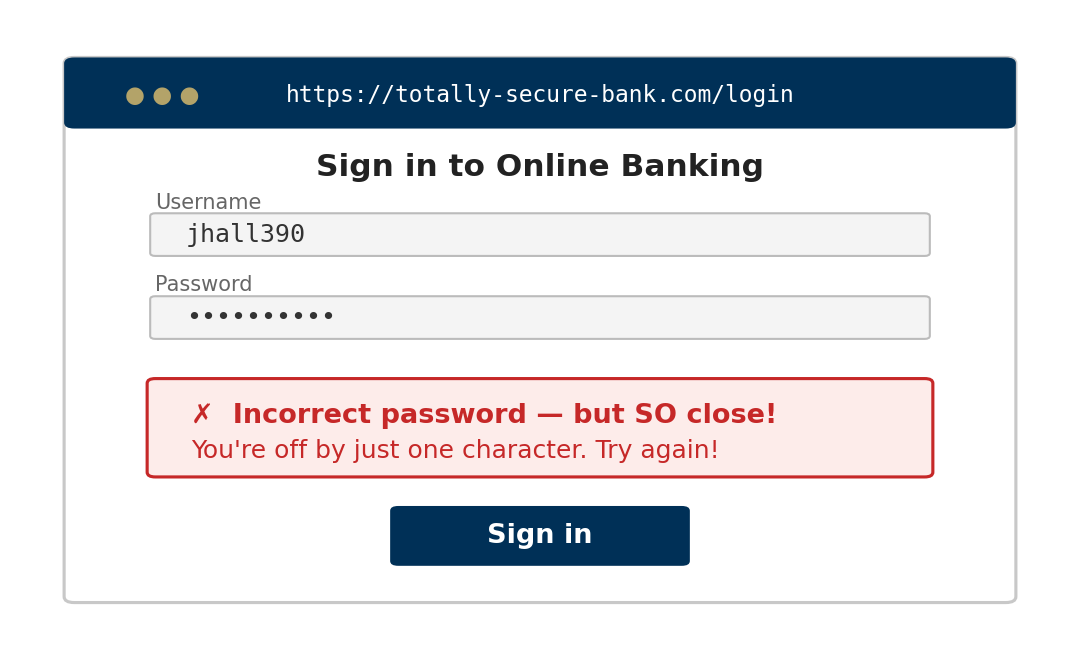
\includegraphics[width=0.56\textwidth]{fig_password_redflag.png}
\end{center}
\pause
\vspace{-1mm}
{\small If the server can tell you are close, it is comparing your guess to your \ul{actual password} -- stored in plain text. A server storing only $H(\text{password})$ cannot know you were off by one character: the hash of $N$ reveals nothing about the hash of $N \pm 1$.}

\end{frame}

\begin{frame}
\frametitle{Hash Functions}

Hash functions are the basis for \textbf{Proof of Work}
\bi
\m By publishing $y=H(x)$, anyone can check that they know the real $x$ without $x$ ever becoming public information \pause 
\bi
\m Easy to compute $H(x)$ given $H(\cdot)$ and $x$ \pause 
\m If someone changes $x$ to $\tilde{x}$, even by one letter, $H(\tilde{x})$ will be very different!
\m Used in checksums for file downloading  
\ei
\m The application we care about is \textbf{mining and proof-of-work}
\bi 
\m No way to discover $x$ given $H(x)$ beside \textbf{brute force}!  
\m The Secure Hash Algorithm 1 (``\textbf{SHA1}'') takes between $2^{63}$ - $2^{80}$ evaluations to find a collision ($x,y$ such that $H(x)=H(y)$) (depending on how clever you are)  
\m Bitcoins are mined by brute-forcing hashes to find $x$s that produce $H(x)$ with leading zeroes. 
\ei 
\ei

\end{frame}

\subsection{Digital Signatures}

\begin{frame}
\frametitle{Digital Signature Schemes}

The requirements are
\bi
\m JPH has a public key everyone knows
\m JPH has a private key only JPH knows
\bi 
\m \textbf{Non-invertability} means the public key doesn't reveal the private key \pause 
\ei 
\m JPH can ``sign'' messages, using the private key to alter the message in a way that proves JPH created his public key 
\m Public key allows \textbf{verification}, but not \textbf{signature production} \pause 
\bi
\m Using the public key, anyone can verify that JPH used his private key to sign the message  
\m But, using the public key, can't generate new valid signatures
\ei
\ei

\end{frame}




\begin{frame}{Digital Signature Schemes, Visually}

\begin{center}
    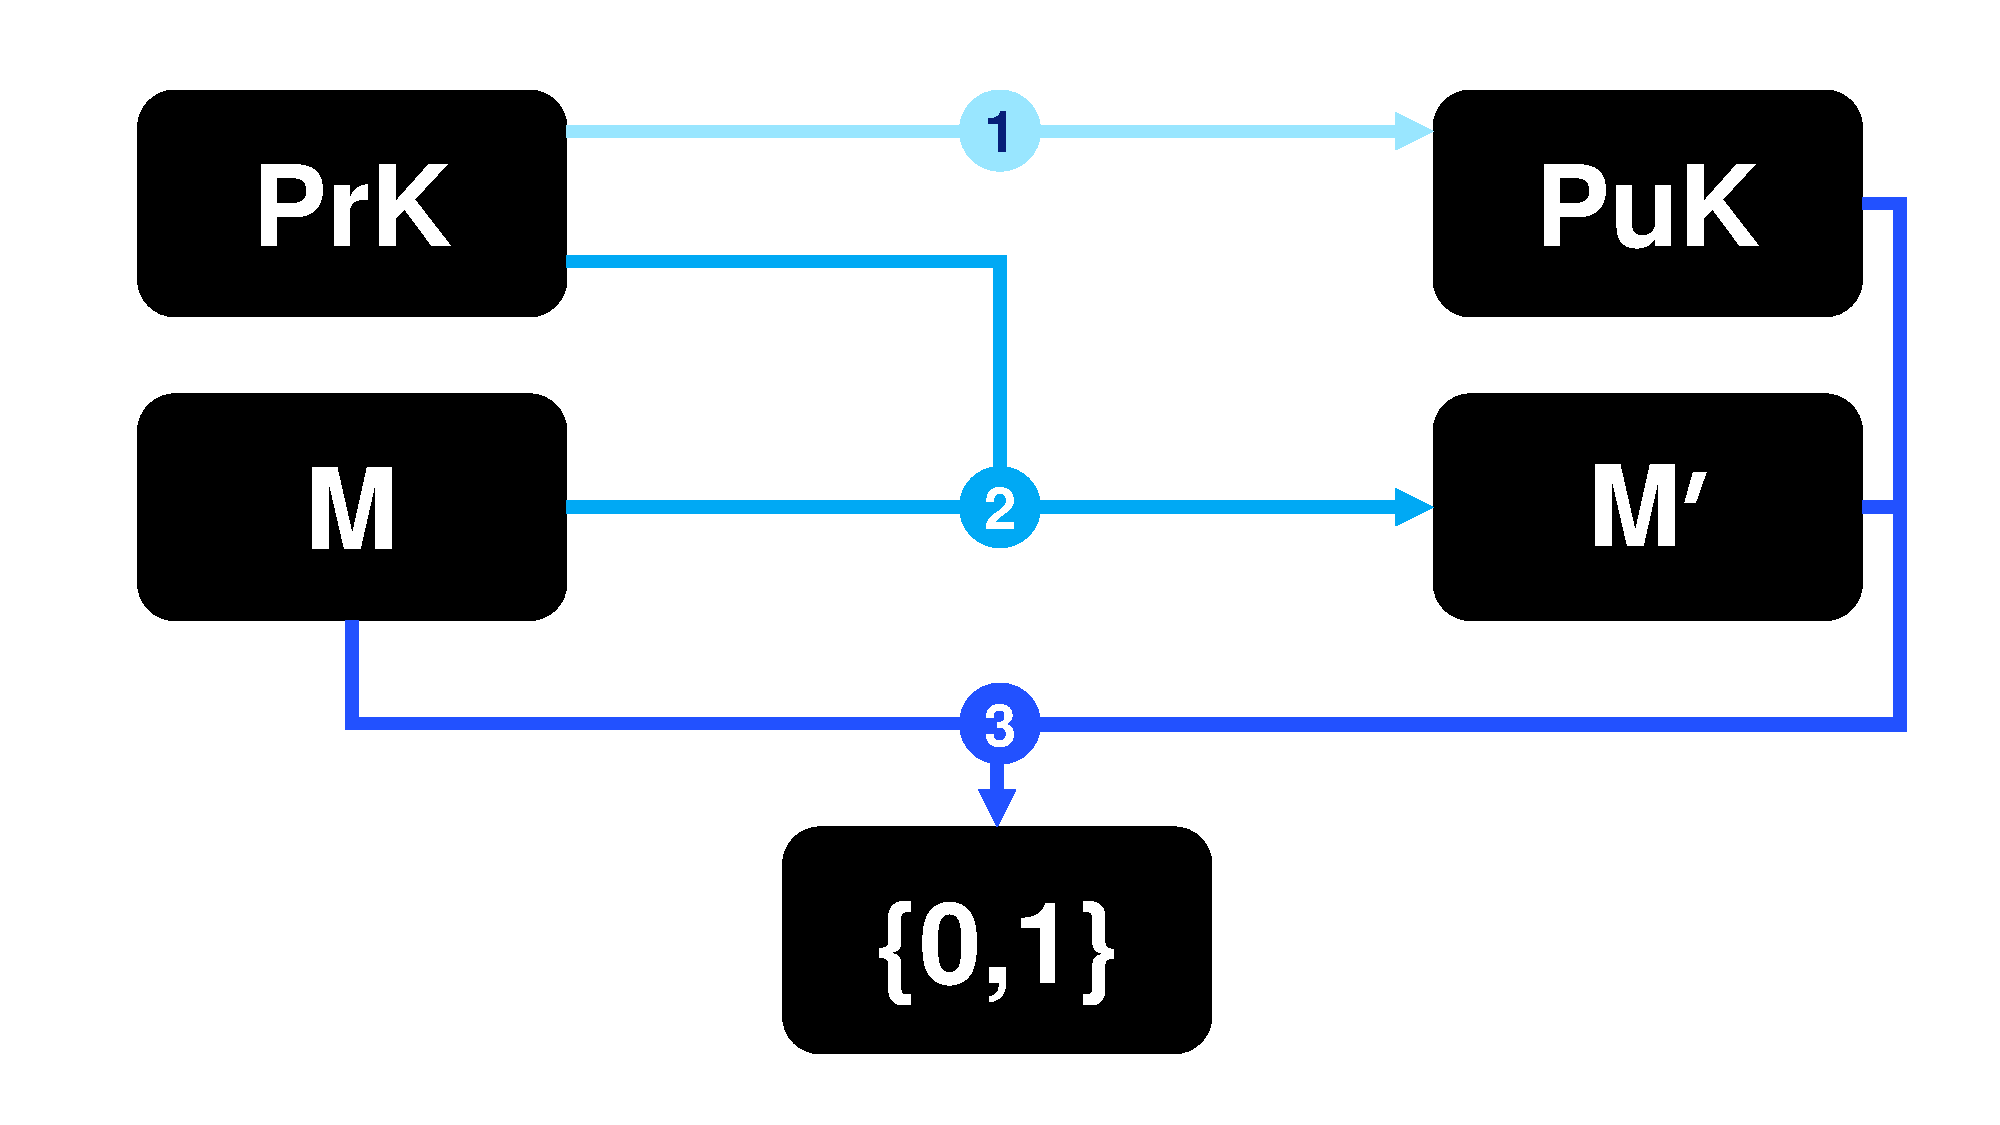
\includegraphics[scale = 0.3]{pics/Financial Technology Timeline for Joseph slide 2.pdf}
\end{center}
    
\end{frame}

\newcommand{\pub}[1]{{\color{blue}#1}}
\newcommand{\priv}[1]{{\color{red}#1}}

\begin{frame}{Clock Arithmetic Is a One-Way Street}

``mod $p$'' means wrap around a clock of size $p$. On a 12-hour clock, $9+4 = 1$. \pause
\bi
\m Do it with \ul{powers}, on a 17-hour clock \ldots
\begin{center}
\begin{tabular}{lccccc}
$3^1, 3^2, 3^3, 3^4, 3^5$ & = & 3, & 9, & 27, & 81, 243 \\
same, mod 17 & = & 3, & 9, & \textbf{10}, & \textbf{13}, \textbf{5} \\
\end{tabular}
\end{center} \pause
\m Without the clock, powers grow in an obvious pattern -- easy to reverse. With the clock, they jump around like random numbers. 
\m One color rule holds for everything that follows. {\color{red}\textbf{Red}} = private; {\color{blue}\textbf{blue}} = public. 
\m Forward is easy. Computing $3^{\priv{d}} \bmod 17$ from $\priv{d}$ is fast, even for enormous $\priv{d}$. 
\m Backward is hopeless. Asked ``which $\priv{d}$ gave me 5?'', you can do no better than trying $\priv{d}$'s one by one. On a 600-digit clock, that outlasts the universe. 
\m This is the \textbf{discrete logarithm problem} -- the one-way street everything below drives on.
\ei

\end{frame}

\begin{frame}{ElGamal, Start to Finish}
\small
\bi
\m \textbf{Setup}: everyone agrees on a clock size $\pub{p}$ and base $\pub{\alpha}$. You pick a secret number $\priv{d}$ and publish
$\pub{\beta} = \pub{\alpha}^{\priv{d}} \bmod \pub{p}$.
Extracting $\priv{d}$ from $\pub{\beta}$ is the discrete log problem, so it is infeasible. \pause
\m \textbf{Sign} a number $\pub{x}$: draw a fresh random $\priv{k}$ and publish $\pub{r}=\pub{\alpha}^{\priv{k}}$; then solve
$\pub{x} = \priv{d}\cdot \pub{r} + \priv{k}\cdot \pub{s}$
for $\pub{s}$ -- the one unknown left -- and publish it. Only someone who \ul{knows} $\priv{d}$ can solve it. \pause
\m \textbf{Verify}: anyone checks, using only blue quantities,
\[ \pub{\beta}^{\,\pub{r}}\cdot \pub{r}^{\,\pub{s}} \;\overset{?}{=}\; \pub{\alpha}^{\pub{x}} \pmod{\pub{p}} \]
\m \textbf{Why it balances}: $\pub{\beta}^{\pub{r}} = \pub{\alpha}^{\priv{d}\pub{r}}$, and the rule $\alpha^{a}\alpha^{b}=\alpha^{a+b}$ still holds on the clock, so the left side is $\pub{\alpha}^{\priv{d}\pub{r} + \priv{k}\pub{s}} = \pub{\alpha}^{\pub{x}}$. \pause
\m \textbf{Why it's secure}: forging $\pub{(r,s)}$ for a new $\pub{x}$ requires knowing $\priv{d}$ -- which is locked behind the one-way street.
\ei

\end{frame}

\begin{frame}{Pop Quiz. What Does This Have to Do With Cryptography?}

\begin{center}
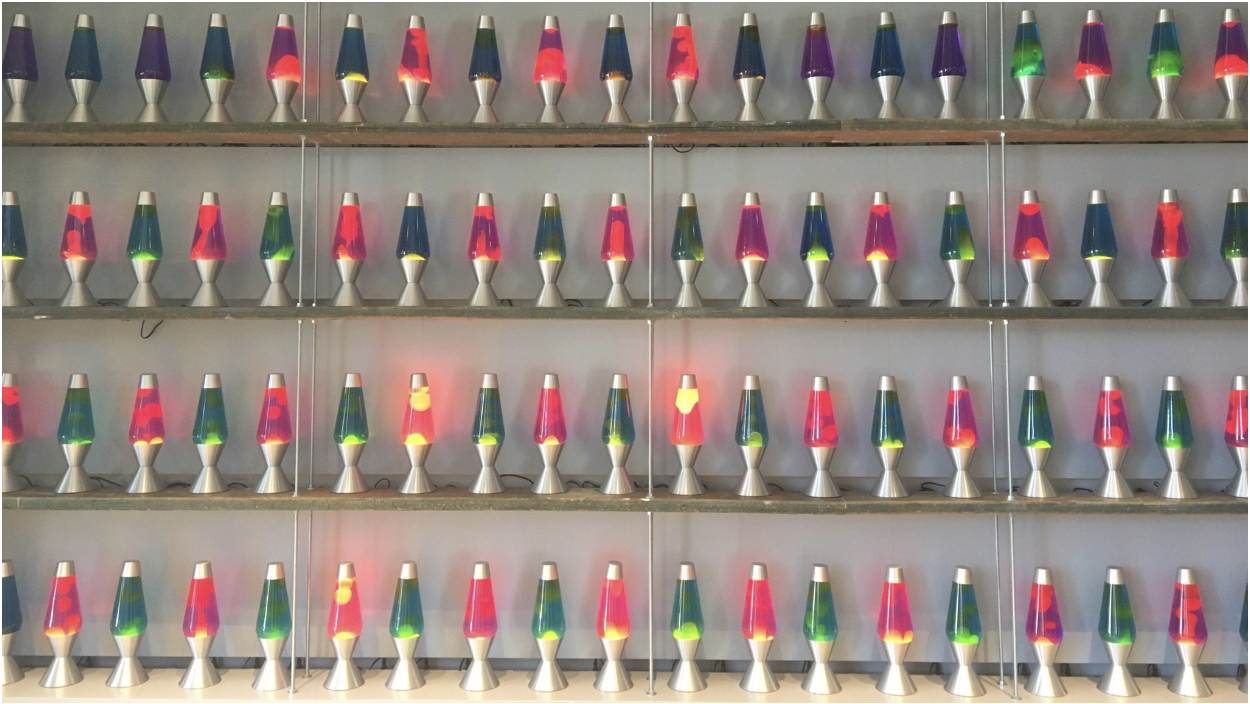
\includegraphics[height=0.8\textheight]{Screenshot 2025-01-28 at 6.23.12 PM.png}
\end{center}

\end{frame}

\begin{frame}{This Wall Helps Encrypt the Internet}

\begin{columns}
\column{0.52\textwidth}
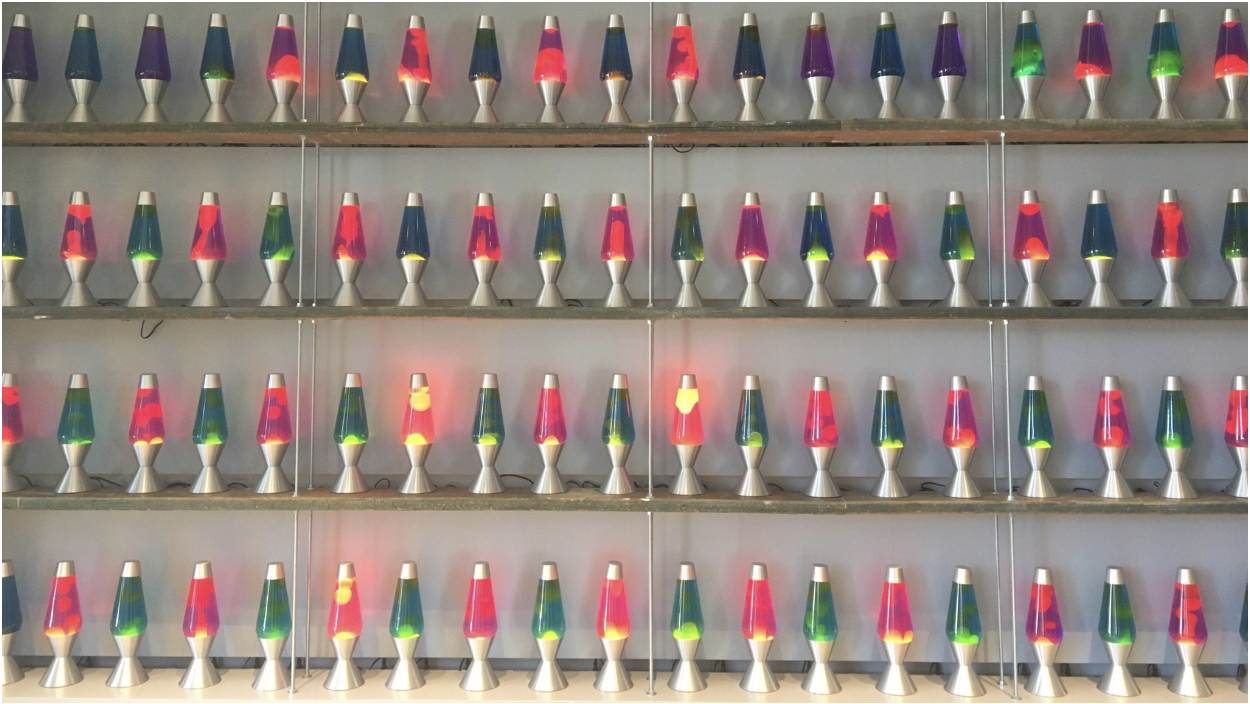
\includegraphics[width=\textwidth]{Screenshot 2025-01-28 at 6.23.12 PM.png}
\column{0.44\textwidth}
\footnotesize
\bi
\m This is the lobby of \textbf{Cloudflare} in San Francisco \pause
\m Every signature needs a fresh, unpredictable $\priv{k}$ -- and computers are terrible at being unpredictable \pause
\m Lava flow is \textbf{chaotic}, deterministic but unpredictable -- the same property we prize in hash functions 
\m A camera films the wall; the pixels help seed the encryption behind https connections at Cloudflare, which fronts \textbf{24.7\% of all websites} (W3Techs, Aug 2026) -- one in four encrypted connections traces randomness to this wall
\ei
\end{columns}

\end{frame}

\begin{frame}{From ElGamal to Digital Signatures}

\bi
\m \ul{Never reuse} $\priv{k}$. Each signature is one equation with two secrets, $\priv{d}$ and $\priv{k}$ -- safely unsolvable. Reuse hands the world two equations in two unknowns, and it solves for $\priv{d}$: Sony's PlayStation~3 signing key fell exactly this way in 2010. \pause

\m $\pub{\beta}$ is the public key everyone knows; $\priv{d}$ is the private key only you know; $\pub{(r,s)}$ is a signature anyone can \ul{verify} from blue quantities alone, but only $\priv{d}$ can \ul{produce}. \pause
\m ElGamal (``The Beauty'' in Arabic) fits in ten lines of Python -- see the \href{https://www.geeksforgeeks.org/elgamal-encryption-algorithm/}{worked code} -- and \href{https://ece.gatech.edu/courses/ece6280}{ECE 6280} goes deeper. Bitcoin uses a cousin (ECDSA) built on the same one-way street.
\ei
\vfill
{\scriptsize The treatment of ElGamal on these slides is adapted from Anthony Lee Zhang's course notes.}

\end{frame}

\subsection{Merkle Trees}

\begin{frame}{Uses of Merkle Trees}

A \hyperlink{https://decentralizedthoughts.github.io/2020-12-22-what-is-a-merkle-tree/}{Merkle Tree} is a way of efficiently storing the required information to ensure that a set of documents or messages have not been tampered with or corrupted. \pause 
\vfill 
Merkle Trees are used in many applications to solve problems such as these.

\bi 
\m Maintaining integrity of files stored on Dropbox.com, or \emph{file outsourcing}
\m Proving a transaction between Alice and Bob occurred, or \emph{set membership}
\m Transmitting files over unreliable channels, or \emph{anti-entropy}
\ei 
    
\end{frame}

\begin{frame}{Construction of Merkle Trees}

Start with, say, 8 files $(f_1...f_8)$, and a hash function $H(.)$ \vfill  

Start by hashing each file, $H(f_i)$ 

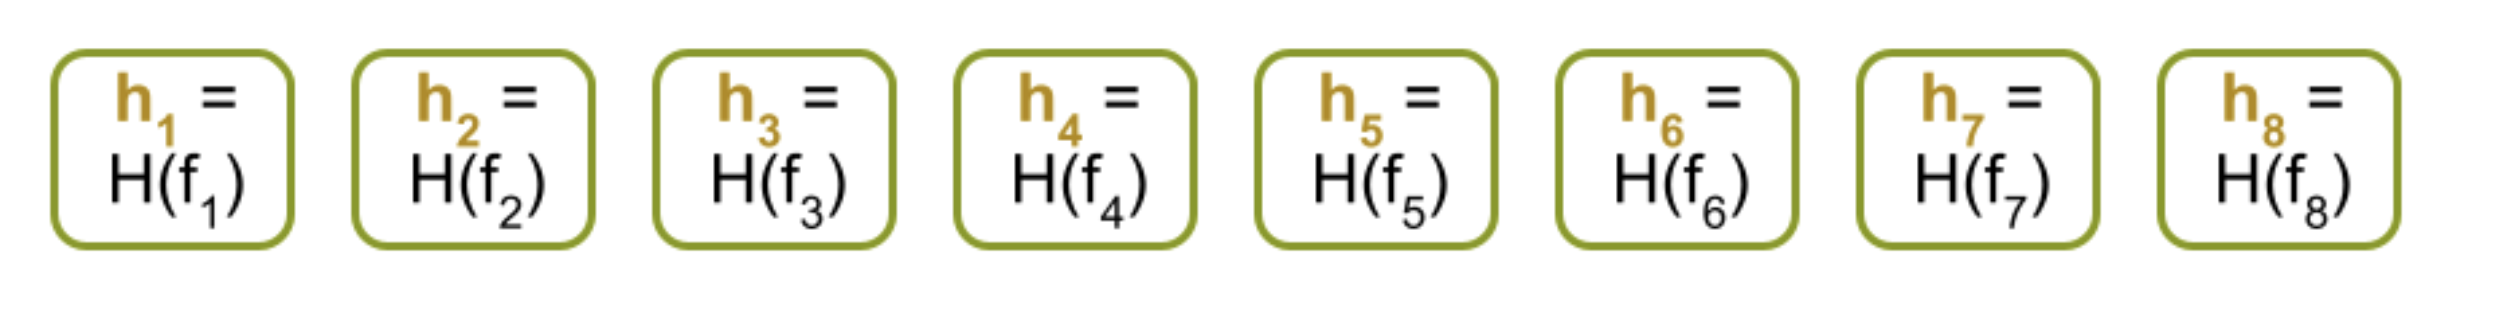
\includegraphics[scale = 0.3]{Screenshot 2025-01-27 at 7.38.00 PM.png}
    
\end{frame}

\begin{frame}{Construction of Merkle Trees}

Next, hash each pair of hashes 

\begin{center}
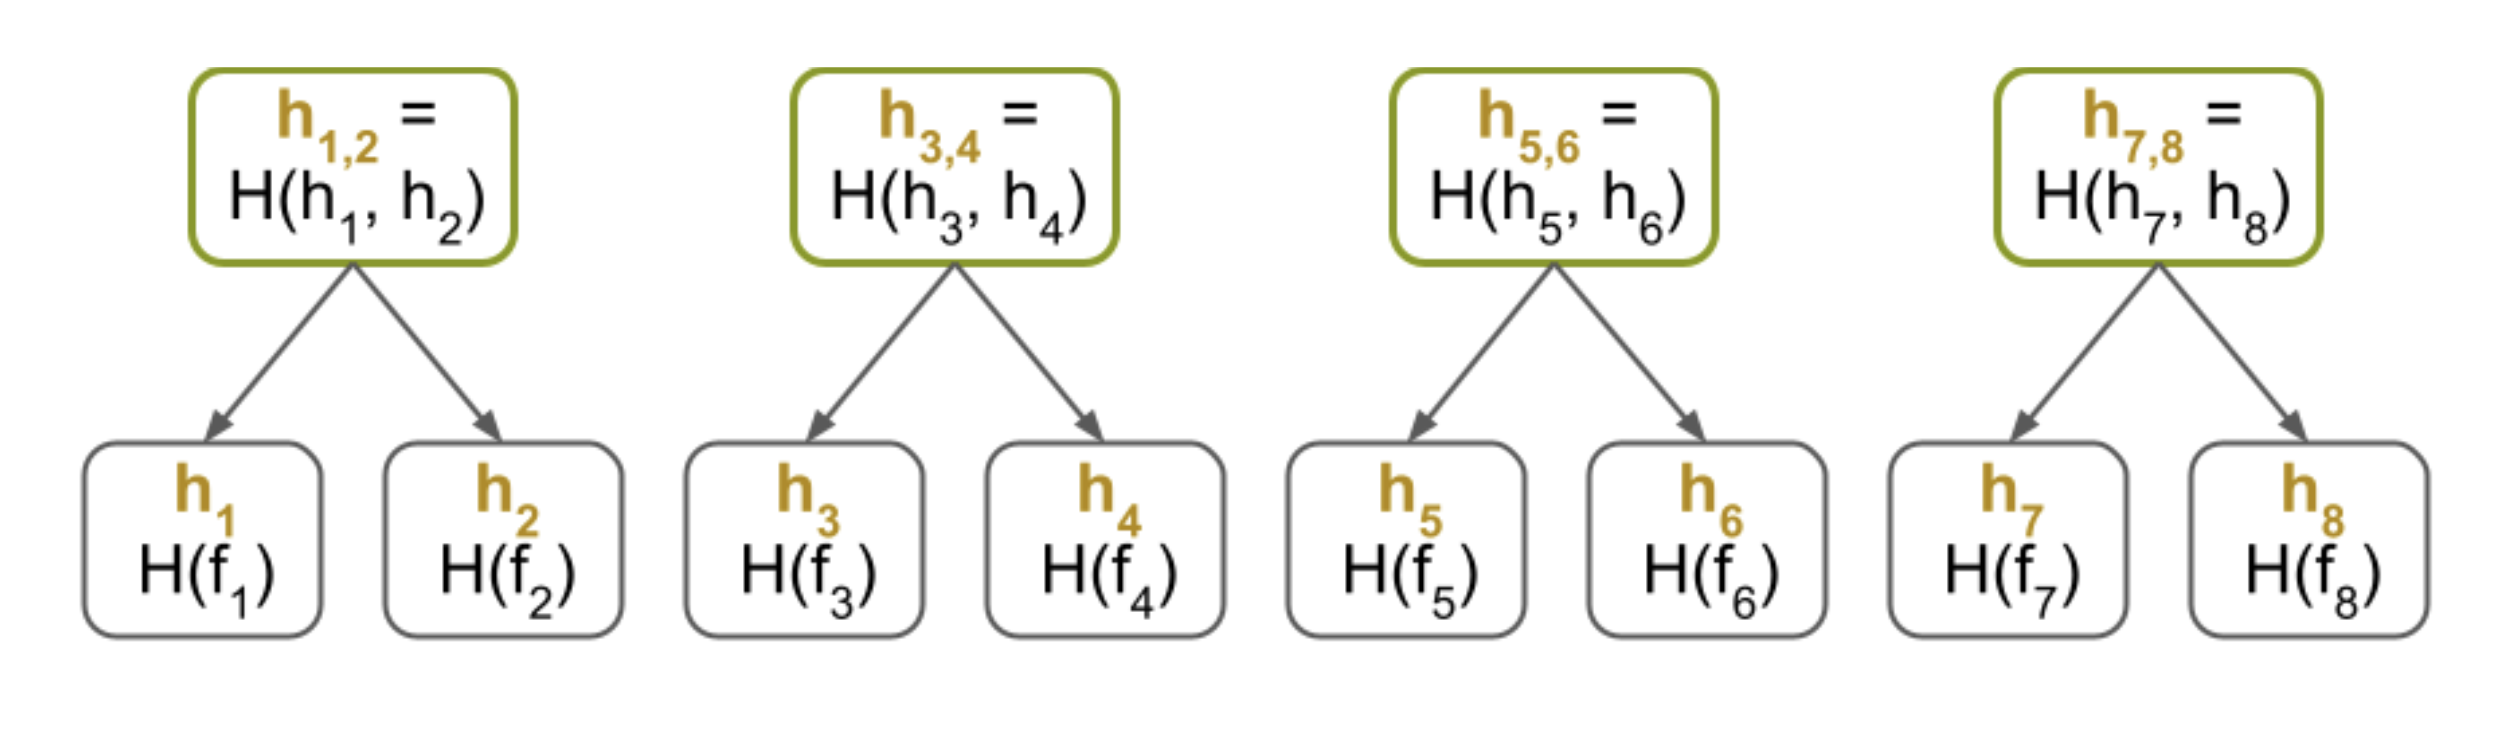
\includegraphics[width = 0.85\textwidth]{Screenshot 2025-01-27 at 7.40.09 PM.png}
\end{center}
    
\end{frame}

\begin{frame}{Construction of Merkle Trees}

Repeat until one hash remains --- the \textbf{Merkle Root} $h_{1,8}$ 

\begin{center}
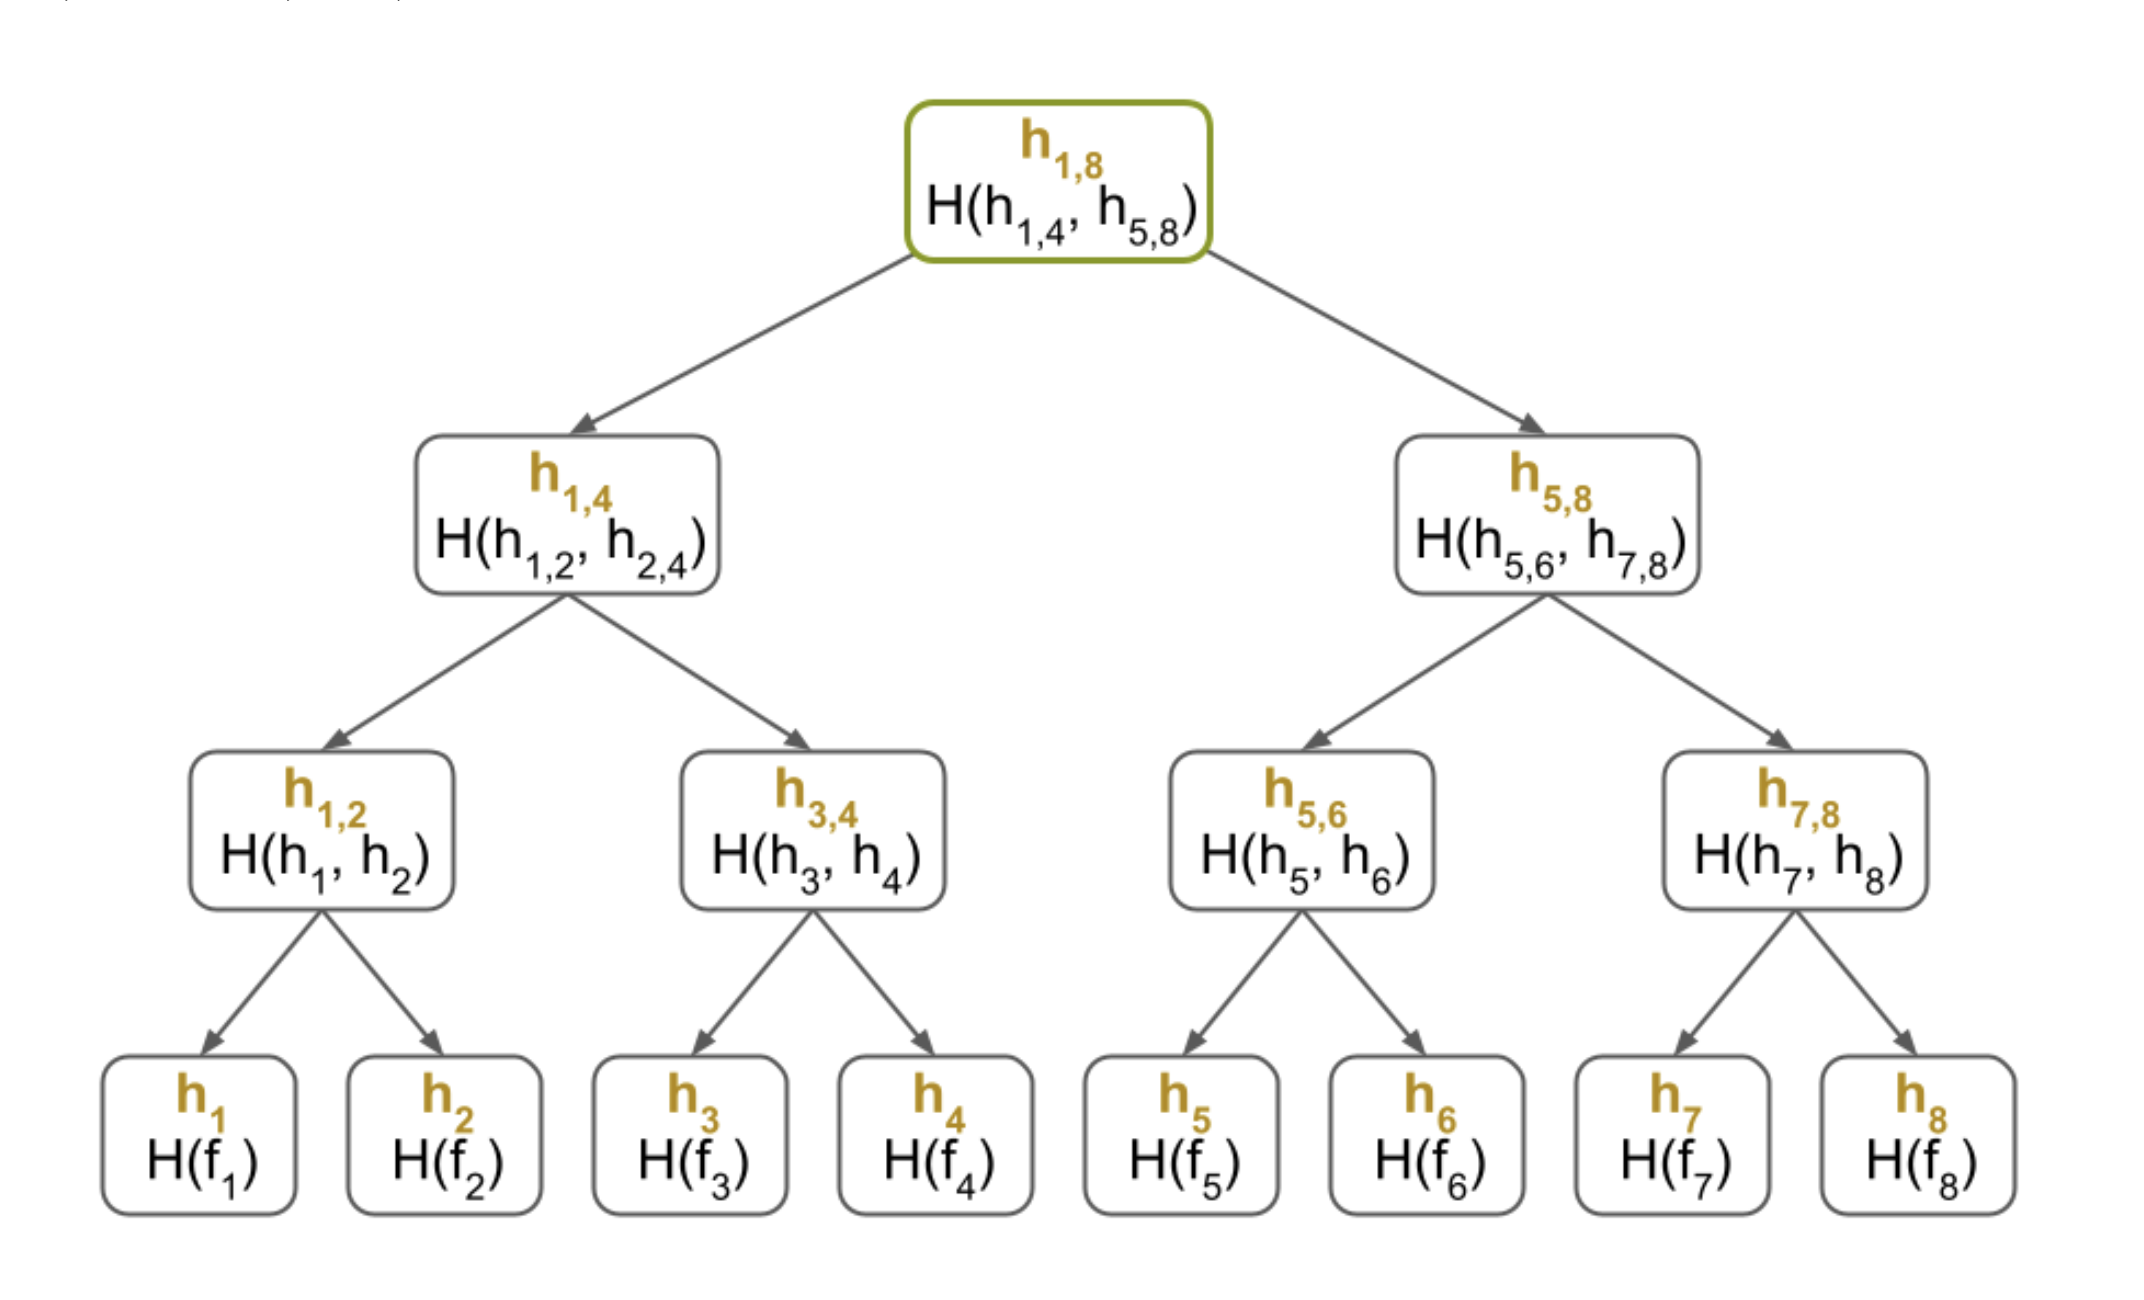
\includegraphics[width = 0.45\textwidth]{Screenshot 2025-01-27 at 7.43.10 PM.png}
\end{center}
\vfill
{\small This building block predates Bitcoin by three decades.}
    
\end{frame}

\begin{frame}{Ralph Merkle}

\begin{center}
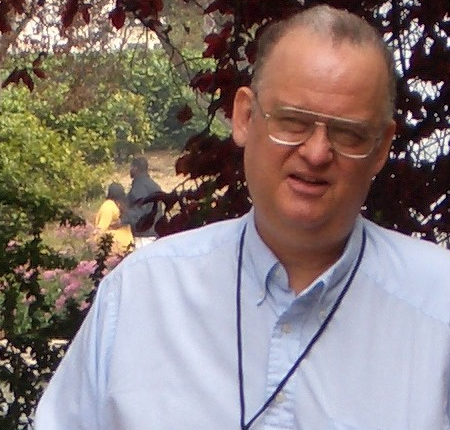
\includegraphics[height=0.68\textheight]{fig_ralph_merkle.jpg}
\end{center}
\vspace{1mm}
{\small Invented the Merkle tree in 1979 --- and was later a \textbf{Georgia Tech professor of computing}. Photo: Wikimedia Commons.}

\end{frame}







\begin{frame}{Verification with Merkle Trees}

Upload your files $(f_1...f_8)$ \textbf{and} your Merkle Tree to Dropbox, storing only the \textbf{Merkle Root} $h_{1,8}$ locally. \pause \vfill 
Later, ask for the file you want, say $f_3$, but make sure to also ask for the \textbf{Merkle Proof}: the hashes needed to compute $h_{1,8}$ from the desired \textbf{Merkle Leaf} ($f_3$) \pause
\vfill
The proof needs only \textbf{one hash per level}, so it scales with $\log_2 n$
\bi
\m 8 files $\rightarrow$ 3 hashes
\m 1{,}024 files $\rightarrow$ 10 hashes
\m \alert{one billion files $\rightarrow$ 30 hashes ($\sim$1 KB)}
\ei

\end{frame}



\begin{frame}{Advantages of Merkle Trees}

\textbf{Question}: Why not just store the hash of every file? Wouldn't that be simpler? \pause \\ 
\textbf{Answer}: That would require storing 1 hash per document, so your local storage would scale linearly with number of files. The Merkle Tree requires storing \textbf{only} the Merkle Root, a single hash, \textbf{for any number of files}! \pause 

\vfill 
\textbf{Question}: The server stores ($h_4$, $h_{1,2}$, and $h_{5,8}$) for you. Can't the server modify these to make the Merkle Proof appear true, even if $f_3$ is changed to $\tilde{f_3}$?    \\ 
\textbf{Answer}: The cryptographic property of \textbf{Non-Invertability} ensures that it is prohibitively difficult to create a false Merkle proof. 
\vfill  
For other (analogous) uses of Merkle Trees including Transaction Verification and Transmitting files robustly over error-prone communication channels, see \hyperlink{https://decentralizedthoughts.github.io/2020-12-22-what-is-a-merkle-tree/}{Tomescu (2020)}
    
\end{frame}


\section{Blockchains}

\subsection{Centralized Blockchain}

\begin{frame}{What is a Blockchain?}

A \textbf{Blockchain} is a list of records that are linked together by hash functions

\begin{center}
    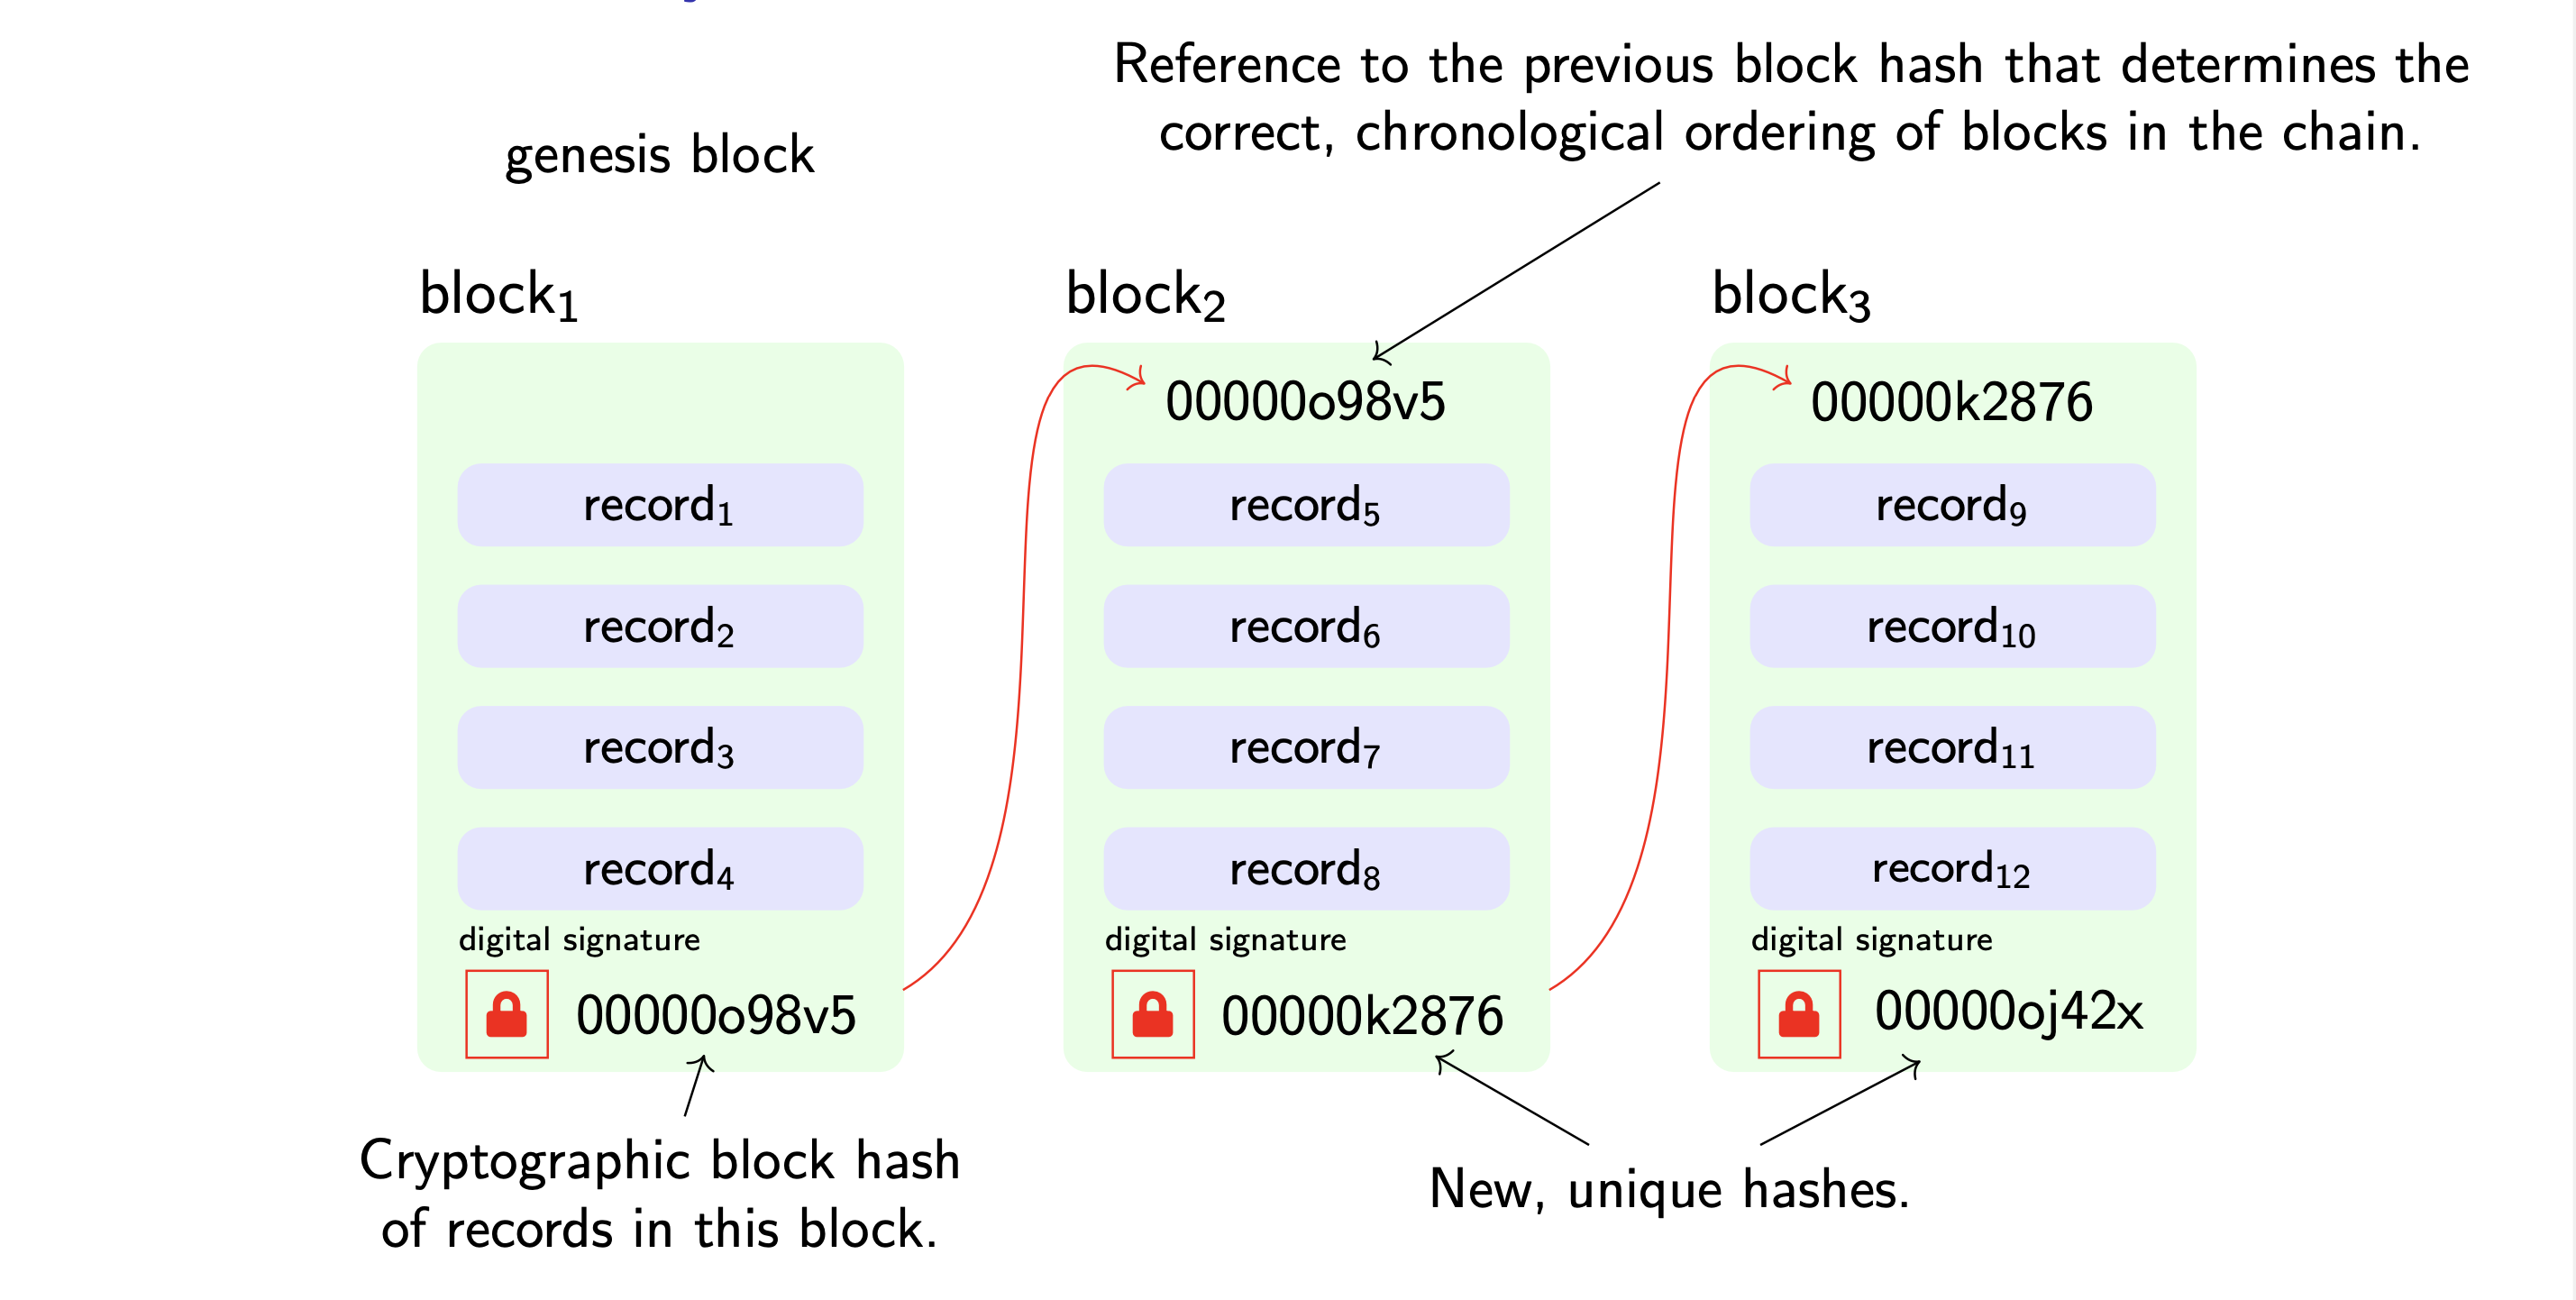
\includegraphics[scale = 0.25]{Screenshot 2025-01-27 at 7.03.18 PM.png}
\end{center}
    
\end{frame}

\begin{frame}{A Centralized Blockchain}

Say that I, JPH, own and operate a private server which records a Blockchain. I don't know the users' private keys, but I control everything that is written on the blockchain. What can I do? \pause 
\begin{itemize}
    \item Create false messages? \pause 
    \bi 
    \m No -- I don't have the private keys to create messages that can be verified as true.  
    \ei 
    \item Cancel or revert messages? 
    \bi 
    \m Yes -- I can refuse to include a new block or roll back the blockchain to a previous state.  
    \ei 
    \item Selectively cancel three messages ago, but not the last two?  
    \bi 
    \m No -- the hashes of the last two messages would be wrong if the middle hash is missing. 
    \ei 
\end{itemize}
    
\end{frame}

\begin{frame}{A Centralized Blockchain}
\small
Centralized Blockchains are in fact widely-used. 

\bi 
\m Binance Smart Chain 
\m Coinbase Base 
\m Ripple XRP 
\m ``Permissioned'' or ``Private'' Blockchains use \textbf{Proof of Authority}, where the admin's public key \emph{per se} is hard-coded into the protocol. 
\ei \pause 
When are these better than just a spreadsheet? \pause \\ 
\bi 
\m Often they aren't. Chase, VISA, Zelle, and Federal Reserves are all just spreadsheets at the end of the day  
\m A Centralized Blockchain adds one extra level of security -- a transaction history that can't be arbitrarily tampered with, only censored or rewound   
\m That's still a lot of power in the admin's hands!
\ei 

\end{frame}


\subsection{Decentralized Blockchain}

\begin{frame}{A Decentralized Blockchain}

\textbf{Can we take away even more power from the admin -- agree on a shared history without trusting anybody?} \pause

\begin{itemize}
    \item  A natural, “democratic” rule would be to have multiple admins taking turns adding transactions to the chain \pause 
    \item How do we prevent one admin from just pretending to be multiple admins?  
    \item Needs to be some “cost”/“barrier” to becoming an admin  
    \item Bitcoin solves this through \textbf{proof of work}
    \item Ethereum solves this through \textbf{proof of stake}
\end{itemize}
    
\end{frame}


\begin{frame}
\frametitle{Hash Puzzles}

\bi
\m The amount of computational power in the world is finite!
\m Let's try to \href{https://emn178.github.io/online-tools/sha256.html}{find a number whose SHA256 hash has a 0 at the beginning}\ldots \pause 
\m Why is this a nice puzzle? Like a PhD
\be
\m Hard to do
\m Proves that you did something hard to do \pause 
\ee
\m With puzzle solution in hand, you become the admin!
\m \textbf{Incentives}. Solving the puzzle earns you BTC, the block reward
\m \textbf{Consensus}. Everyone works on the longest chain 
\bi
\m Cooperating beats defecting to a chain of your own, because when compute is power you want to be on the side with the most compute
\ei 
\ei

\end{frame}






\section{Bitcoin}

\subsection{History}

\begin{frame}
\frametitle{Satoshi Nakamoto}

\bi
\m Started sending emails about Bitcoin August 2008
\m The Bitcoin \href{https://bitcoin.org/bitcoin.pdf}{white paper} and code appeared in October 2008
\m The first block was mined on January 9!
\bi
\m ``The Times 03/Jan/2009 Chancellor on brink of second bailout for banks''
\ei
\m On May 22, 2010, Laszlo Hanyecz bought two Papa John's pizzas for 10,000 BTC, now worth \$600mil USD!
\m Quickly became popular among black markets, \href{https://en.wikipedia.org/wiki/Silk_Road_(marketplace)}{Silk Road}\ldots
\bi
\m Founder Ross Ulbricht was recently pardoned by Trump 
\ei
\ei
	
\end{frame}

\begin{frame}
\frametitle{Prizes for a Starcraft Tournament in 2011}

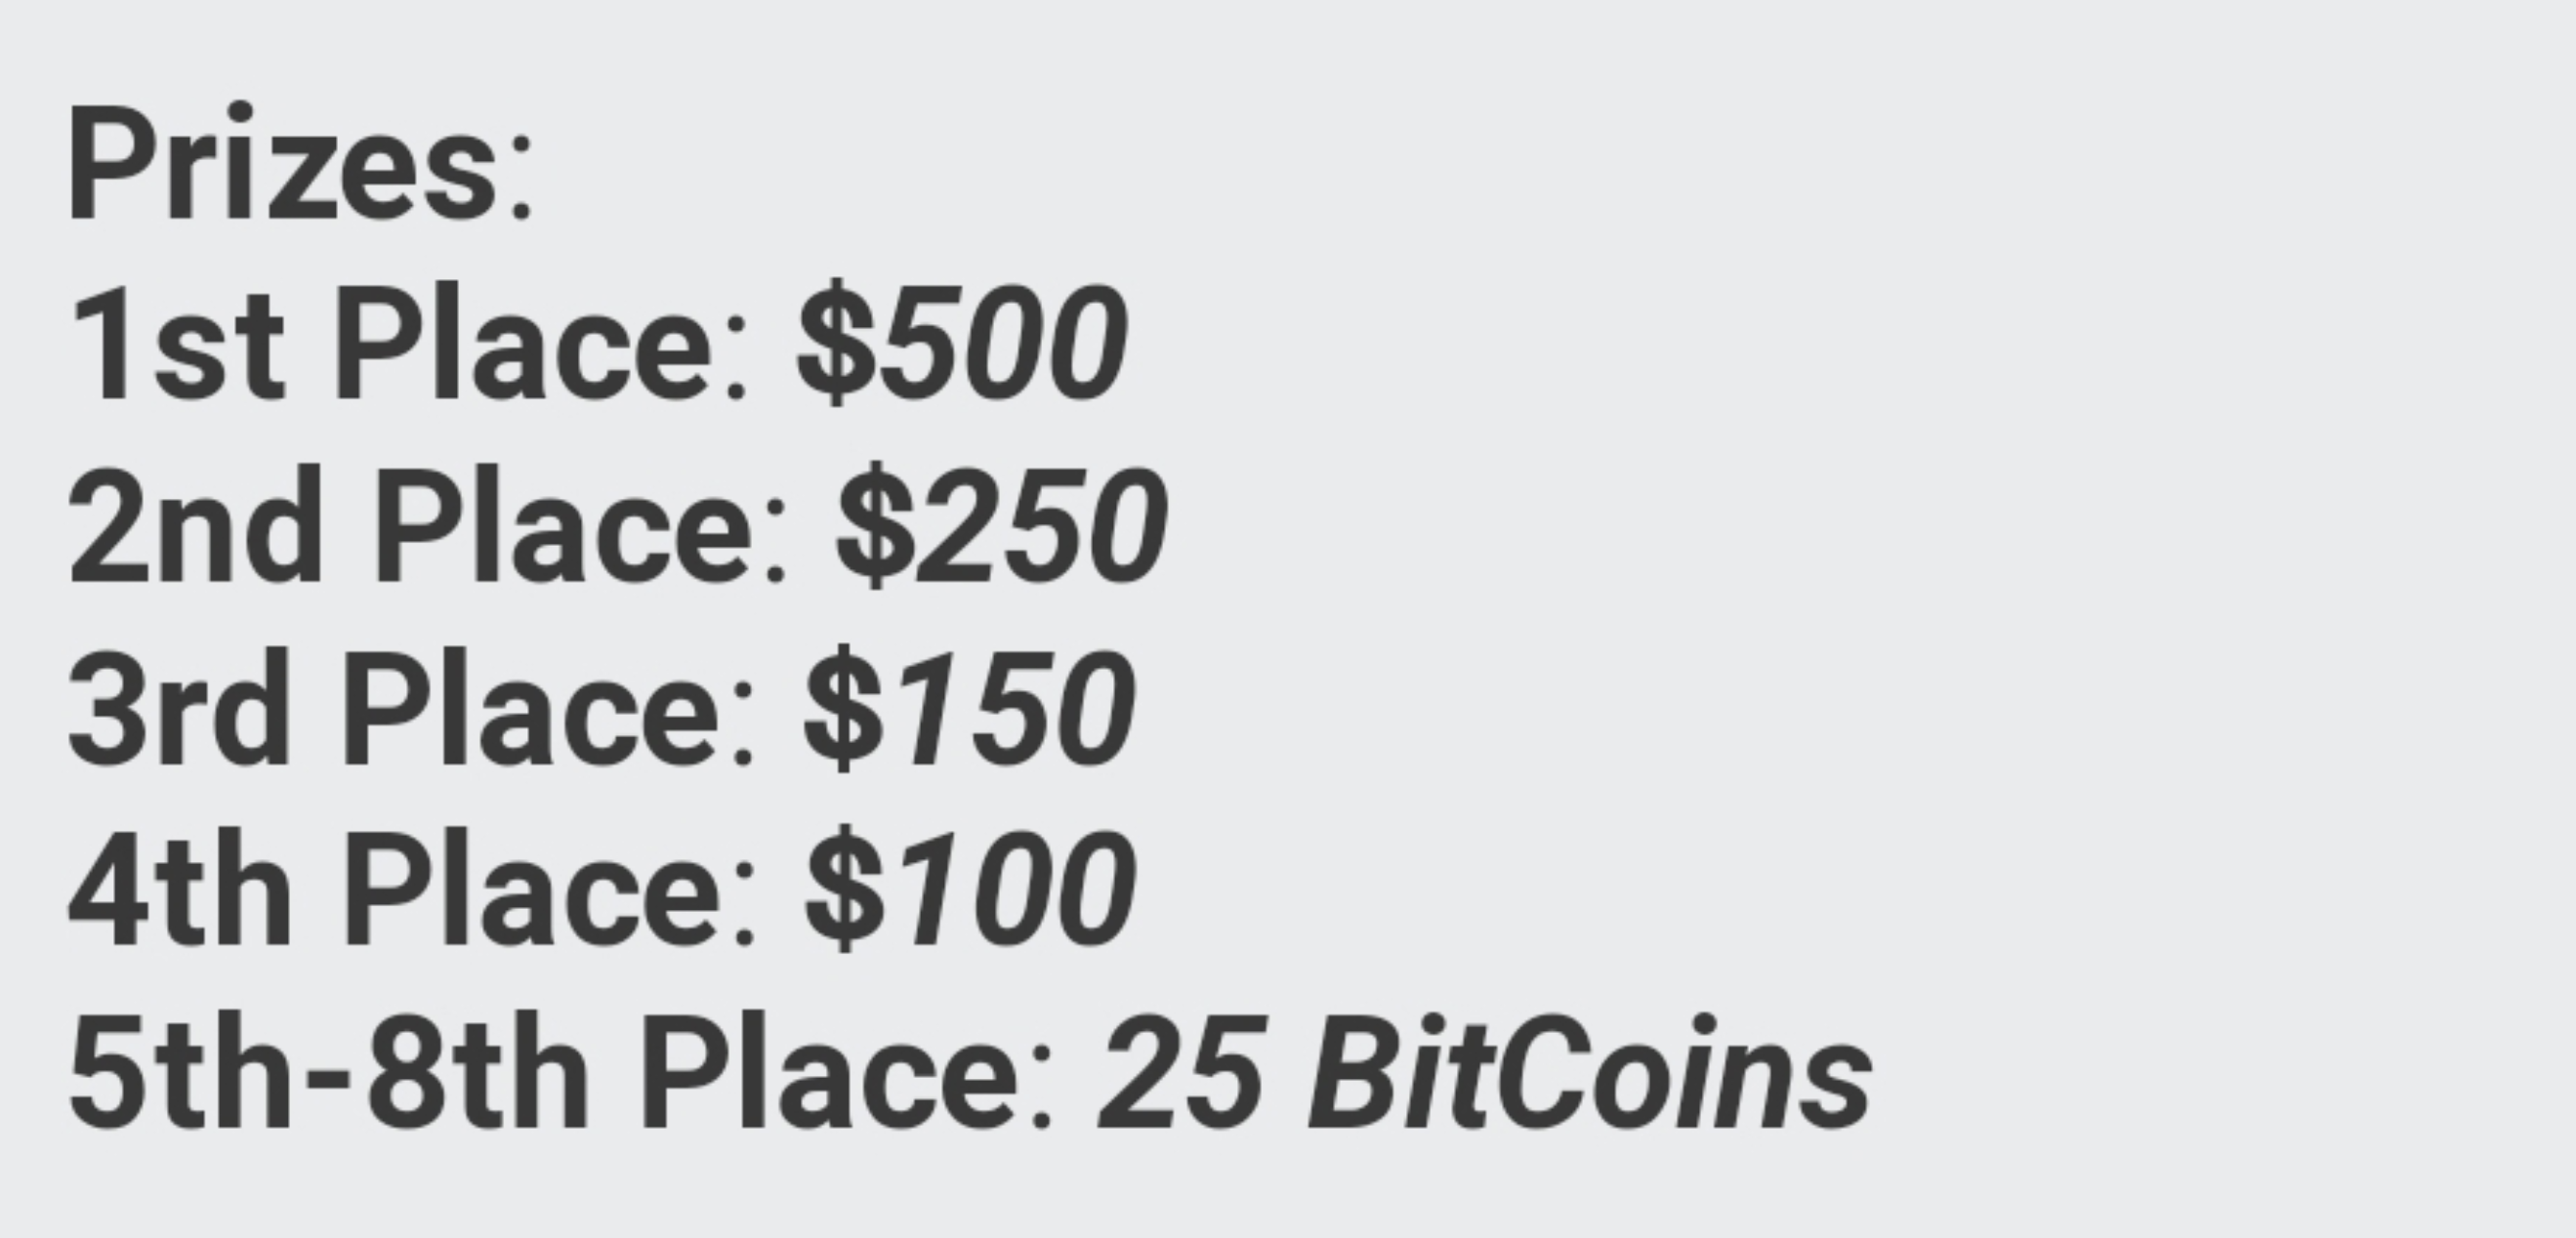
\includegraphics[height = 0.8\textheight]{Screenshot 2025-01-28 at 3.03.46 PM.png}
    
\end{frame}

\begin{frame}
\frametitle{Bitcoin Prices}

\begin{center}
\href{https://coinmarketcap.com/currencies/bitcoin/}{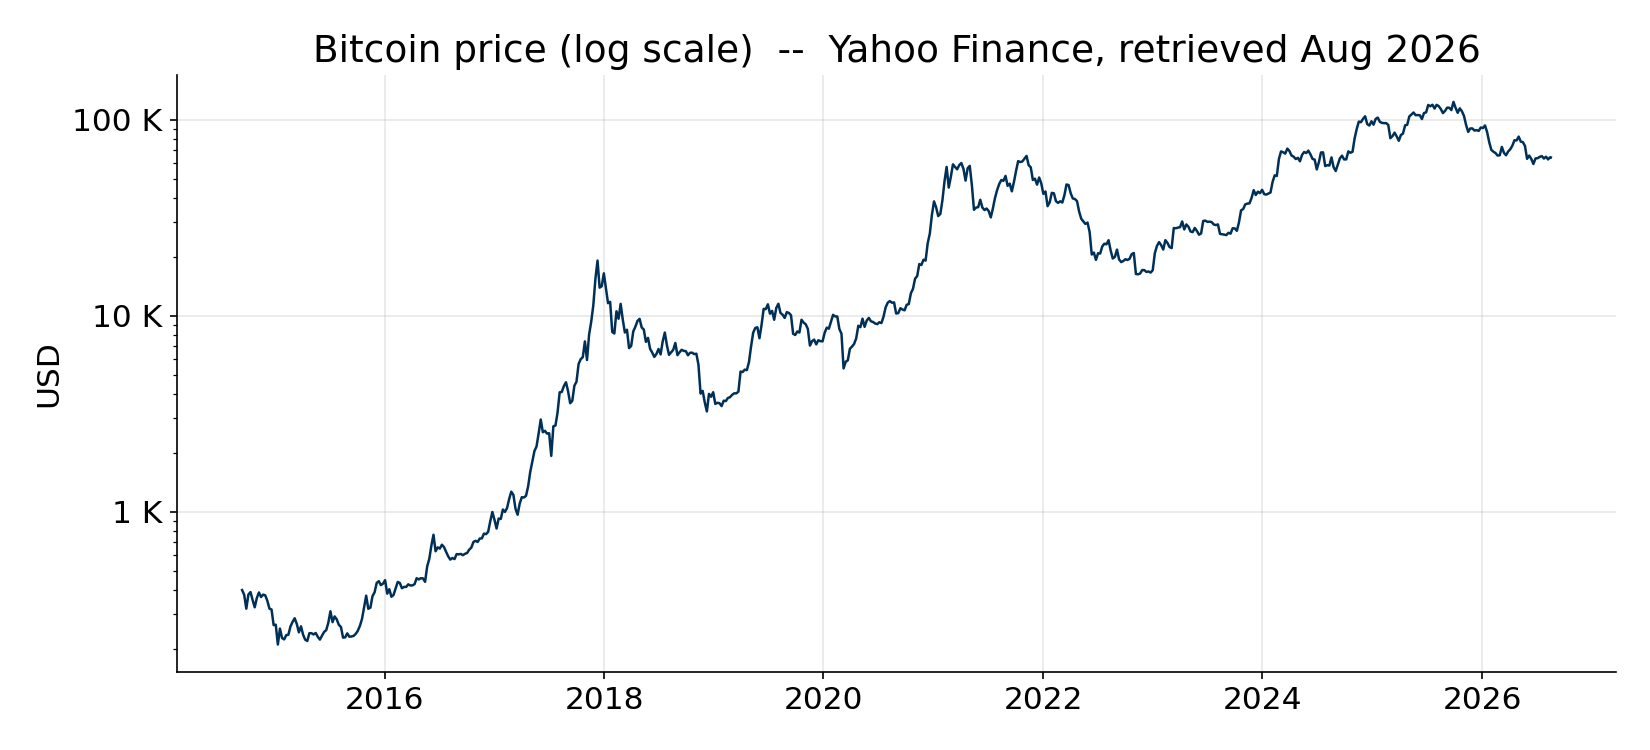
\includegraphics[width = .8\textwidth]{fig_btc_price_full.png}}
\end{center}

\scriptsize
\href{https://finance.yahoo.com/quote/BTC-USD/}{Yahoo Finance}, retrieved Aug 2026 (chart is clickable -- live version)

\end{frame}

\subsection{Structure}

\begin{frame}
\frametitle{Each BTC Block is a Merkle Tree of Transactions!}

\begin{center}
	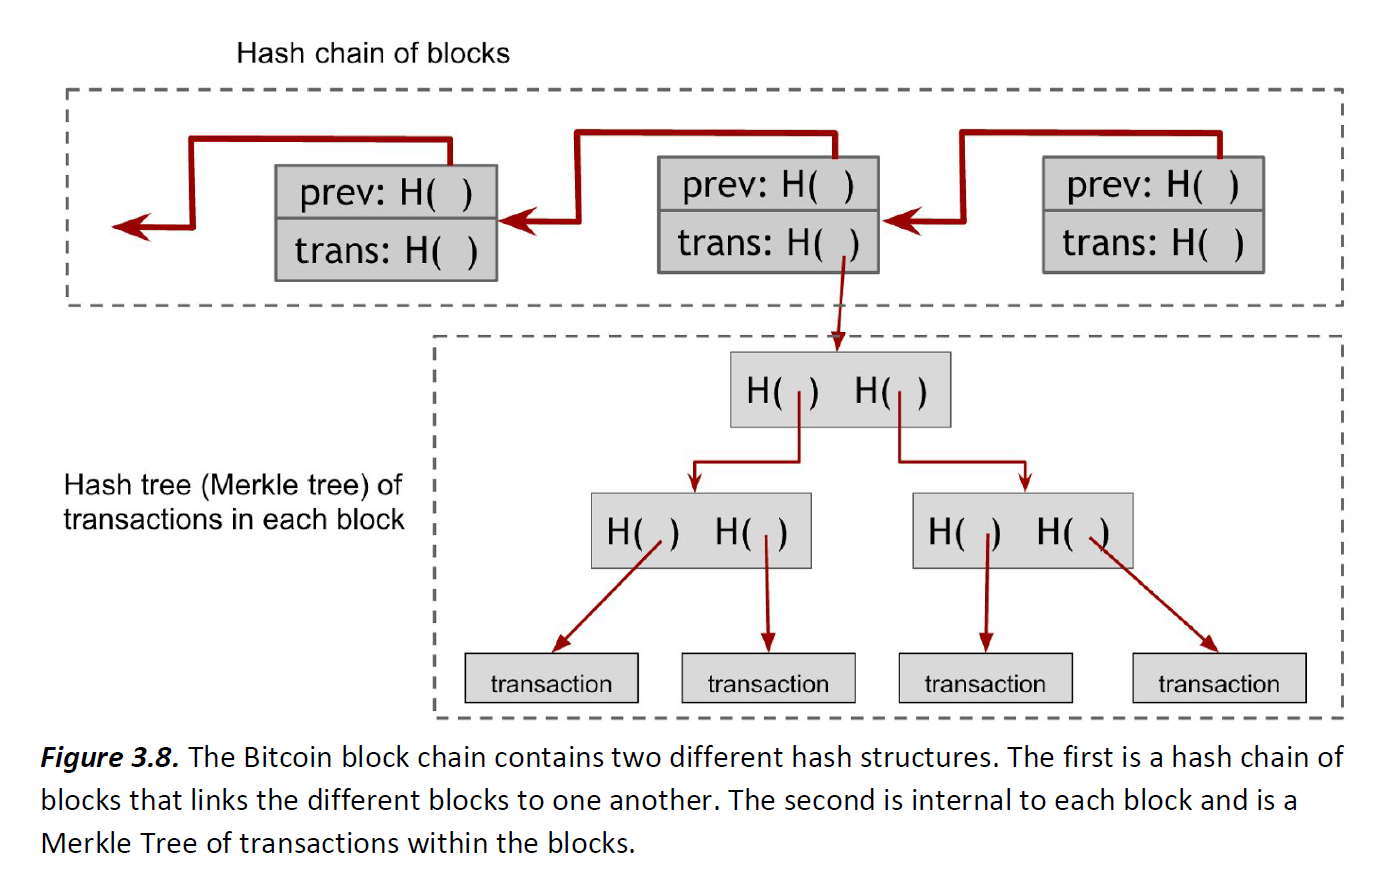
\includegraphics[width = 0.58\textwidth]{pics/blockchain_book.png}
\end{center}

\bi
\m Valid block headers' hashes start with a big number of 0's (mining puzzle)
\ei

\vspace{2ex}

\scriptsize

\href{https://d28rh4a8wq0iu5.cloudfront.net/bitcointech/readings/princeton_bitcoin_book.pdf?a=1}{NBFMG}, fig. 3.8

\end{frame}








\subsection{Long-Run Dynamics}




\begin{frame}
\frametitle{BTC mining}

\bi
\m Suppose mining a block pays 0.001 BTC
\m Suppose mining block costs \$60 in electricity
\bi
\m If BTC price $>\$60k$, everyone mines; blocks produced quickly
\m If BTC price $<\$60k$, nobody mines; tx's aren't included and the blockchain stops working!
\ei
\m The fact that mining rate depends on BTC vs electricity price is not desirable\ldots
\m The fix is difficulty adjustment, which maintains a constant block production rate
\ei

\end{frame}

\begin{frame}
\frametitle{BTC Difficulty Adjustment}

\bi
\m Blocks should be produced every 10 minutes
\m Every 2016 blocks (approx 14 days), Bitcoin considers average block production rate, and\ldots
\bi
\m Increases/decreases hash problem difficulty, if block production is too fast/slow
\ei
\m What determines how fast blocks are produced, fixing hash rate? \pause
\bi
\m How many people (that is, how much electricity) is devoted to mining
\ei \pause
\m What determines how many people mine?
\bi
\m How profitable mining is, that is, how high BTC price is, vs electricity price
\ei
\ei

\end{frame}




\begin{frame}
\frametitle{The Money Pot Game}

\bi
\m You have two options.
\be
\m Get \$1 for sure
\m Fight for a \$10 pot, which is equally divided between everyone who picks this option
\ee \pause
\m Which do you pick?
\ei

\end{frame}

\begin{frame}
\frametitle{The Money Pot Game}

\bi
\m What is going on?
\bi
\m Everyone wants the money pot
\m But the more people take the money pot, the less money there is for everyone
\m In ``Nash equilibrium'', the money pot becomes no better than the ``outside option''
\ei \pause
\m What's the equilibrium condition in similar settings?
\bi
\m Firms competing for profits? \pause
\m Going to the beach on a sunny day? 
\m Getting a table for Brunch on Sunday at 12pm? 
\ei
\m ``Equilibrium'' behavior is easy to predict in such settings
\bi
\m In equilibrium, the ``good'' deal is so crowded that it becomes just as bad as the ``bad'' deal
\ei 
\m Game theory calls these \ul{congestion games}, or \ul{wars of attrition}, or \ul{tragedy of the commons}
\ei

\end{frame}

\begin{frame}
\frametitle{Difficulty vs BTC price}

\begin{center}
\href{https://www.blockchain.com/explorer/charts/difficulty}{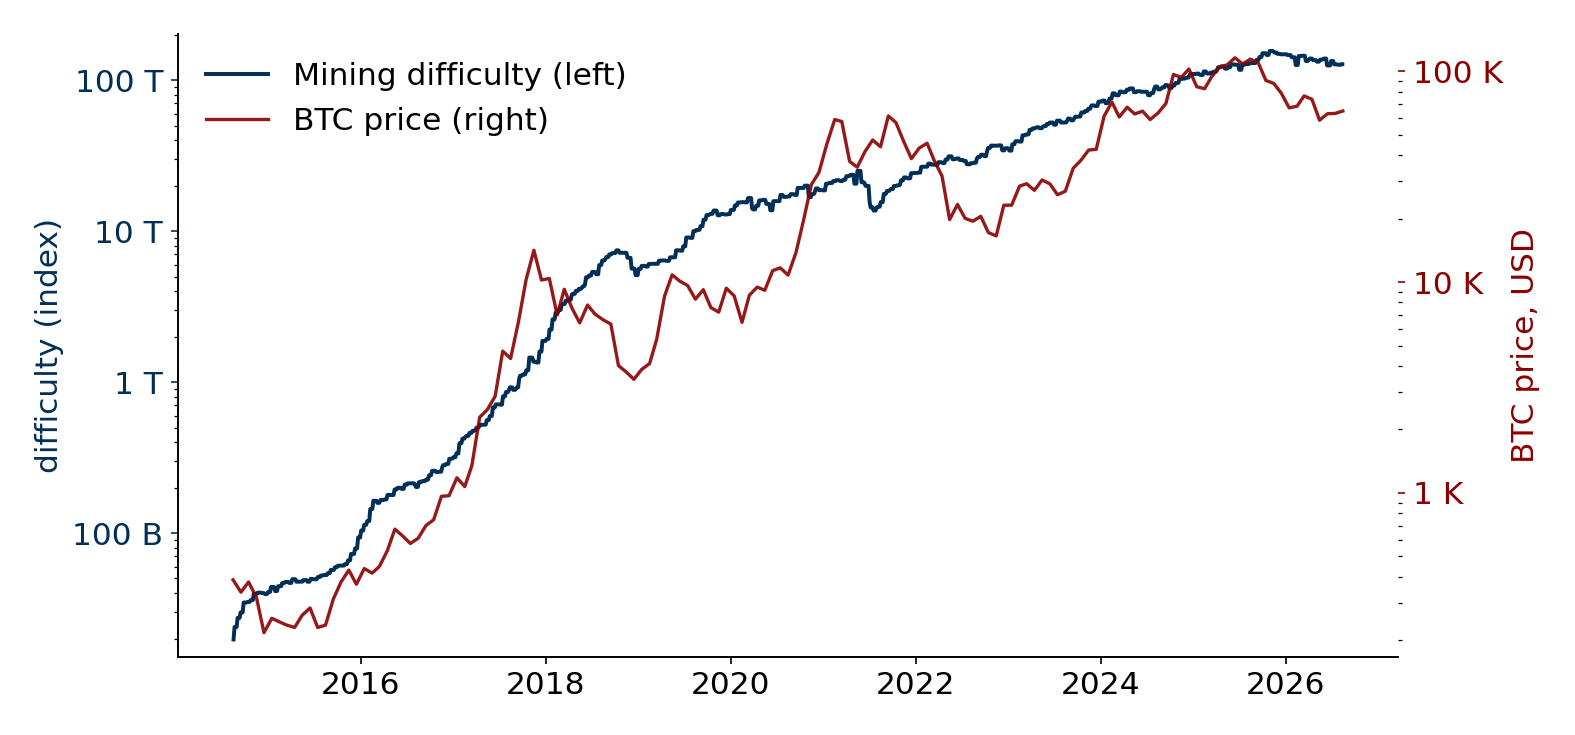
\includegraphics[width = .85\textwidth]{fig_btc_difficulty.png}}
\end{center}


\scriptsize
Difficulty is an index, where $1$ = the first block (January 2009) and today $\sim$127 trillion. \href{https://www.blockchain.com/explorer/charts/difficulty}{Blockchain.com}, Aug 2026 (chart is clickable -- live version)

\end{frame}





\begin{frame}
\frametitle{BTC Halving}

\bi
\m Approximately every 4 years, issuance of BTC drops by half
\m The last halving was April 2024, leaving 3.125 BTC per block
\m Does this affect block production rate?
\bi
\m No! Difficulty adjustment always ensure a constant block production rate. 
\ei \pause
\m Also implies there will only ever be 21 million BTC in existence!
\bi 
\m By approximately 2140, the block reward will drop to less than the smallest unit of bitcoin ($1/10^8$) and become equal to zero. 
\m Difficulty adjustment ensures that block production rate is approximately constant 
\ei 
\ei

\end{frame}

\begin{frame}
\frametitle{Bitcoin Is Digital Gold -- Which Is the Problem}
\begin{center}
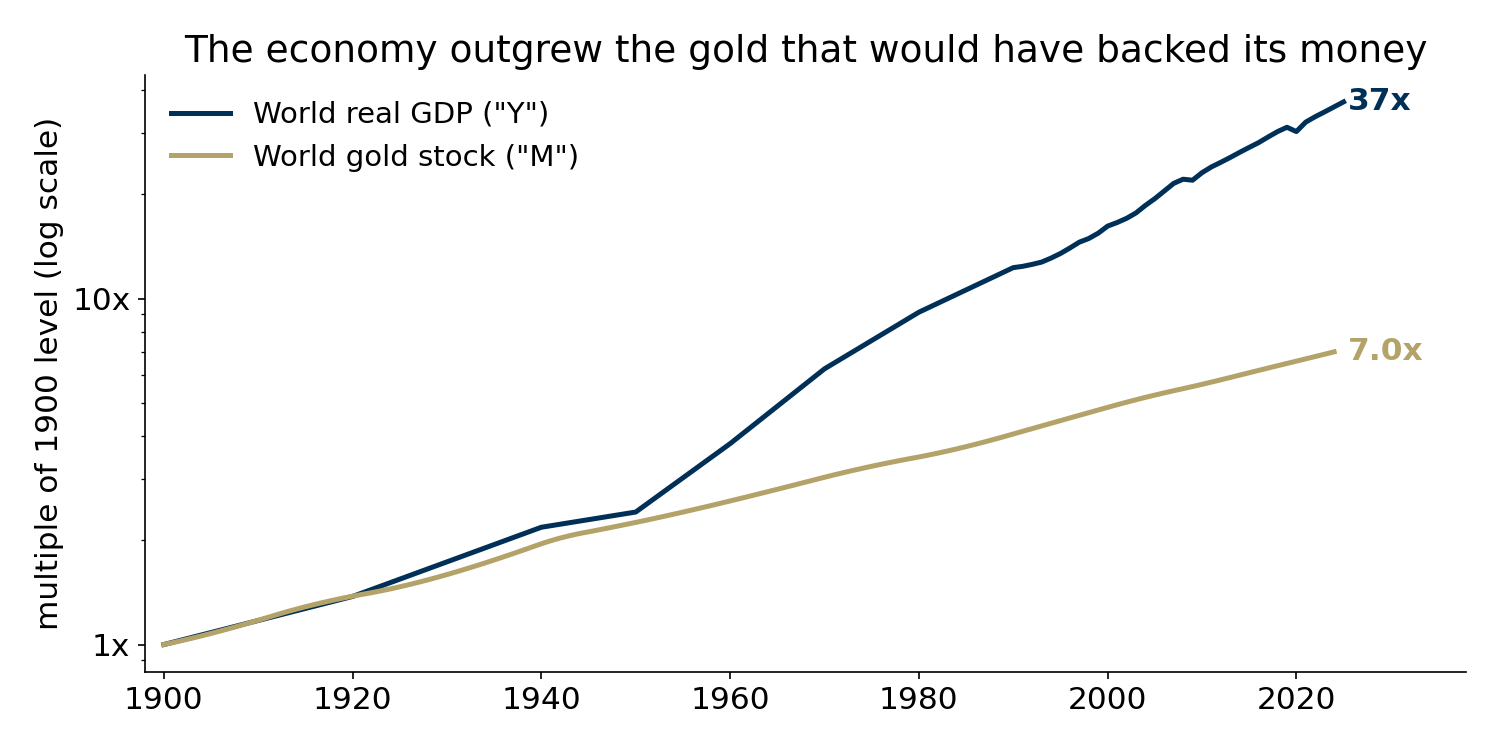
\includegraphics[width=0.7\textwidth]{fig_gold_vs_gdp.png}
\end{center}
\vspace{-1mm}
{\small A hard-capped money supply in an exponentially growing economy forces \textbf{deflation} -- gold's fatal flaw as a currency. Bitcoin's 21M cap is stricter still -- past 2140, its supply stops growing entirely. A plausible store of value; a poor medium of exchange and unit of account.}
\end{frame}

\begin{frame}
\frametitle{Two Meanings of ``Inflation''}

\bi
\m Crypto engineers use ``inflation'' for growth in the \textbf{money supply} -- Ethereum's issuance schedule, Bitcoin's halvings \pause
\m Economists use it for growth in the \textbf{price level} \pause
\m The chart you just saw is where the two definitions part ways. Zero supply inflation in a growing economy is not zero price inflation -- it is \textbf{deflation}, and deflation punishes borrowers, wages, and anyone who owes a fixed debt
\ei

\end{frame}


\begin{frame}{Transaction Fees}
\small
\bi 
\m Block rewards are not the only incentive -- miners also collect transaction fees, quoted in Satoshis ($10^{-8}$ BTC) per byte; the \textbf{mempool} is the pool of transactions waiting to be included 
\m Fees are also Bitcoin's exit ramp from 2140. When the block reward halves to zero, \textbf{100\% of miner revenue will be fees} -- and maybe that's enough to keep the chain secure 
\ei
\begin{center}
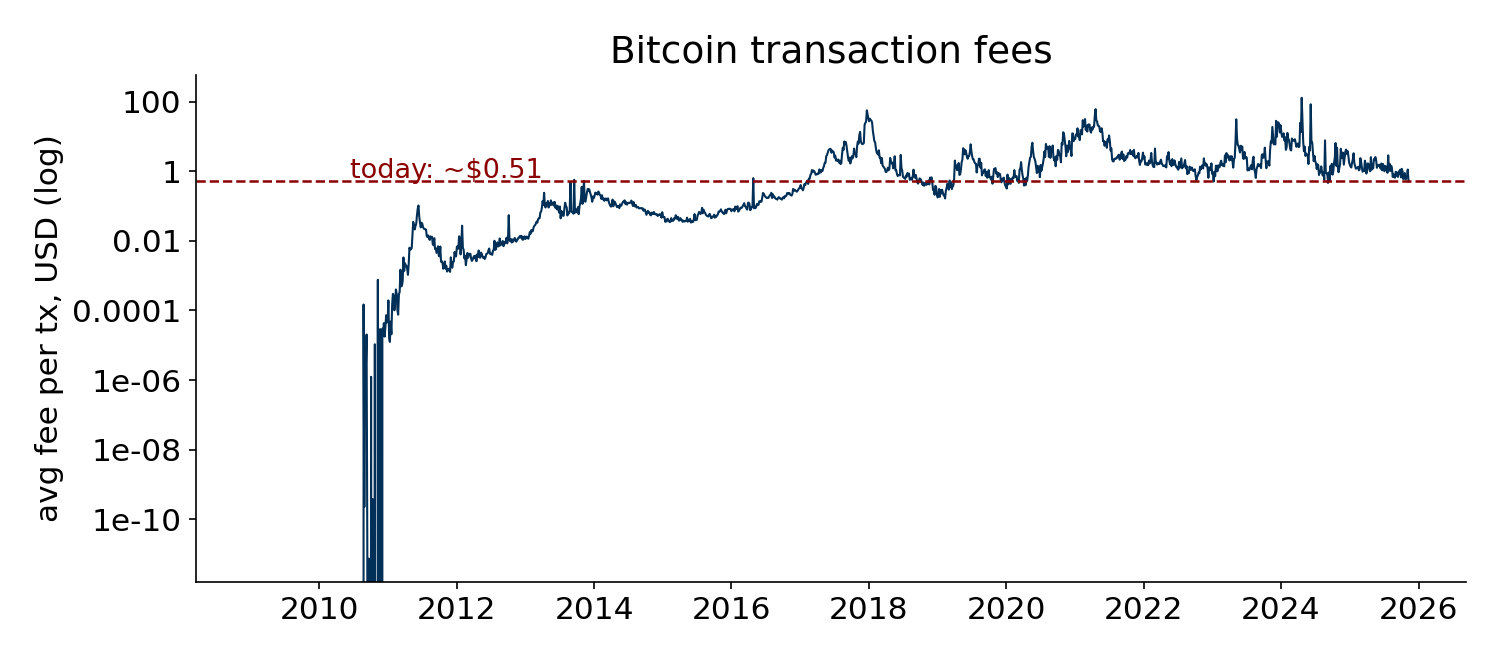
\includegraphics[width=0.60\textwidth]{fig_btc_fees.png}
\end{center}
\vspace{-2mm}
{\small Today an average transaction clears for $\sim$\$0.51. Explore it live at \href{https://mempool.space/}{mempool.space}}
    
\end{frame}




\begin{frame}
\frametitle{Incentives}

\bi
\m A centralized authority can ``censor'', i.e. not include tx's
\m Decentralization and competition ``ensure'' performance
\bi
\m If you don't include my tx, the next miner will
\m Even if the US bans US miners from including tx's, someone else will include them
\ei
\ei

\end{frame}


\begin{frame}
\frametitle{Further Reading on Mining Industry}

\bi
\m Galaxy digital \href{https://www.galaxy.com/insights/research/2023-mid-year-mining/}{2023} and \href{https://www.galaxy.com/insights/research/2024-mid-year-mining/}{2024}
\m Cool \href{https://zhiguohe.net/wp-content/uploads/2023/12/10914-hhaa040.pdf}{paper} on mining pools
\ei

\end{frame}


\section{Ethereum}

\subsection{Smart Contracts}




\begin{frame}
\frametitle{Smart Contracts}

\bi
\m A smart contract is three things.
\bi
\m A wallet, which can hold Ether (ETH),
\m Functions it can call when requested as determined by its code,
\m (optionally) a source of data to which it can read and write \pause 
\ei
\m If you've heard of object oriented programming, smart contracts are a bundle of functions (code), data, as well as ETH balances \pause
\m The most popular coding language which compiles Ethereum script code (a minimal Turing-complete language akin to assembly) is called \textbf{Solidity}  
\ei
Deploying a smart contract or calling its functions requires a \textbf{gas fee} -- ETH must be paid to the network to run the code. 

\end{frame}

\begin{frame}
\frametitle{Smart Contracts Make Tokens}

\bi
\m An ETH address, ``technically'', only ``holds'' Ether (``ETH'') natively -- no other tokens!
\m An ETH address can be assigned non-ETH tokens through smart contracts
\m A smart contract can define tokens using the \textbf{ERC-20} standard 
\bi 
\m So-called because it was originally the 20th submission to ``Ethereum Requests for Comments'' 
\ei 
\ei

\end{frame}


\begin{frame}{Unlike BTC, ETH has native gas fees}

``In Bitcoin, there are no mandatory transaction fees. Transactions can optionally include fees which are paid to miners, and it is up to the miners to decide what fees they are willing to accept. In Bitcoin, such a mechanism is already imperfect\ldots In Ethereum, because of its Turing-completeness, a purely voluntary fee system would be catastrophic. Instead, Ethereum will have a system of mandatory fees, including a transaction fee and six fees for contract computations.'' \\

-Ethereum Whitepaper, Vitalik Buterin (2014)
    
\end{frame}




\subsection{Proof of Stake}

\begin{frame}
\frametitle{Proof of Stake}

\bi
\m Originally, ETH mining proof-of-work, similar to BTC
\m On Sept 15 2022, ETH switched to proof of stake -- called \textbf{``The Merge''}
\m Reduced energy consumption by \textbf{over 99\%}! 
\m Users deposit (``stake'') 32 ETH into a special smart contract
\m Stakers randomly selected (prop. to stake) to propose new blocks
\m If a staker is caught trying to do ``bad things'' (e.g. propose 2 inconsistent blocks), they are ``slashed'' -- staked ETH is removed by smart contract
\m Most newer blockchains (SOL, LUNA, AVAX) use proof-of-stake
\ei

\end{frame}

\begin{frame}
\frametitle{Capacity of Ethereum}

\bi
\m Ethereum L1 processed $\sim$15 transactions per second (tps) for years; staged gas-limit raises have pushed it to $\sim$25 tps today
\begin{center}
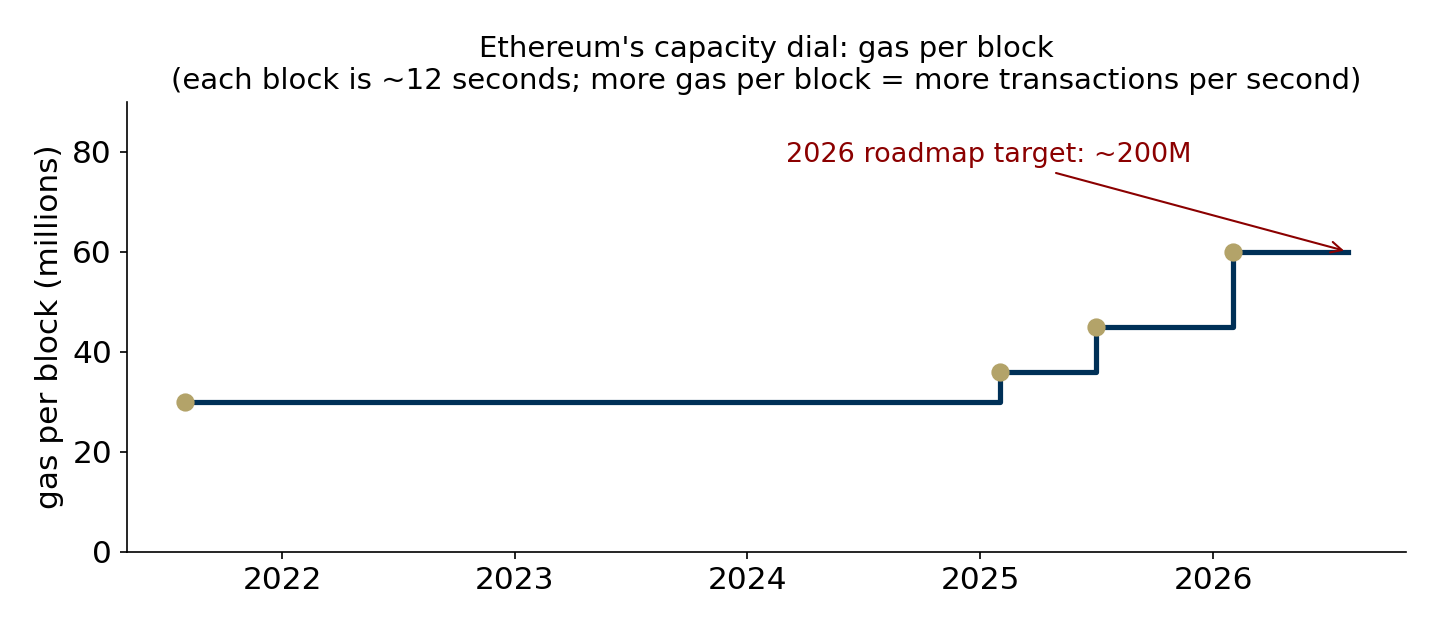
\includegraphics[width=0.56\textwidth]{fig_gas_limit.png}
\end{center}
\m This is pretty bad! Visa is \href{https://crypto.com/university/blockchain-scalability}{24,000 tps}!
\bi
\m Every ETH staker has to run every transaction, and keep a copy of all data!
\ei
\m Decentralization very expensive, in terms of computational efficiency!
\m Proof-of-stake doesn't help throughput
\bi 
\m Rollups do, which we will cover 
\ei 
\ei

\end{frame}


\section{Rollups}

\begin{frame}
\frametitle{Rollups or ``L2's''}
\small
ETH is getting expensive! One set of solutions is \ul{rollups}, also called \ul{L2's}. The idea is this.
\bi
\m Put our ETH, tokens, etc. in a ``smart contract pot'' (L2 bridge)
\m People do transactions (smart contract, etc.) using funds in the pot, without doing anything on ``main chain"
\m Transactions are periodically batch settled \pause
\m Need to guarantee whatever happens on the rollup is exactly what would happen on ETH main chain! There are two methods \pause
\bi
\m An \textbf{optimistic rollup} (Optimism, Arbitrum, Coinbase Base) lets anyone ``challenge'' L2 transactions, will (essentially) run on L1 if challenged
\m In a \textbf{ZK-rollup} (zkSync, StarkWare, Polygon), zero-knowledge cryptographic proofs ensure security, but at a high computing cost
\ei 
\m Optimistic rollups hold the larger market share; ZKs are growing
\ei

\end{frame}

\begin{frame}
\frametitle{L2s Today}
\begin{center}
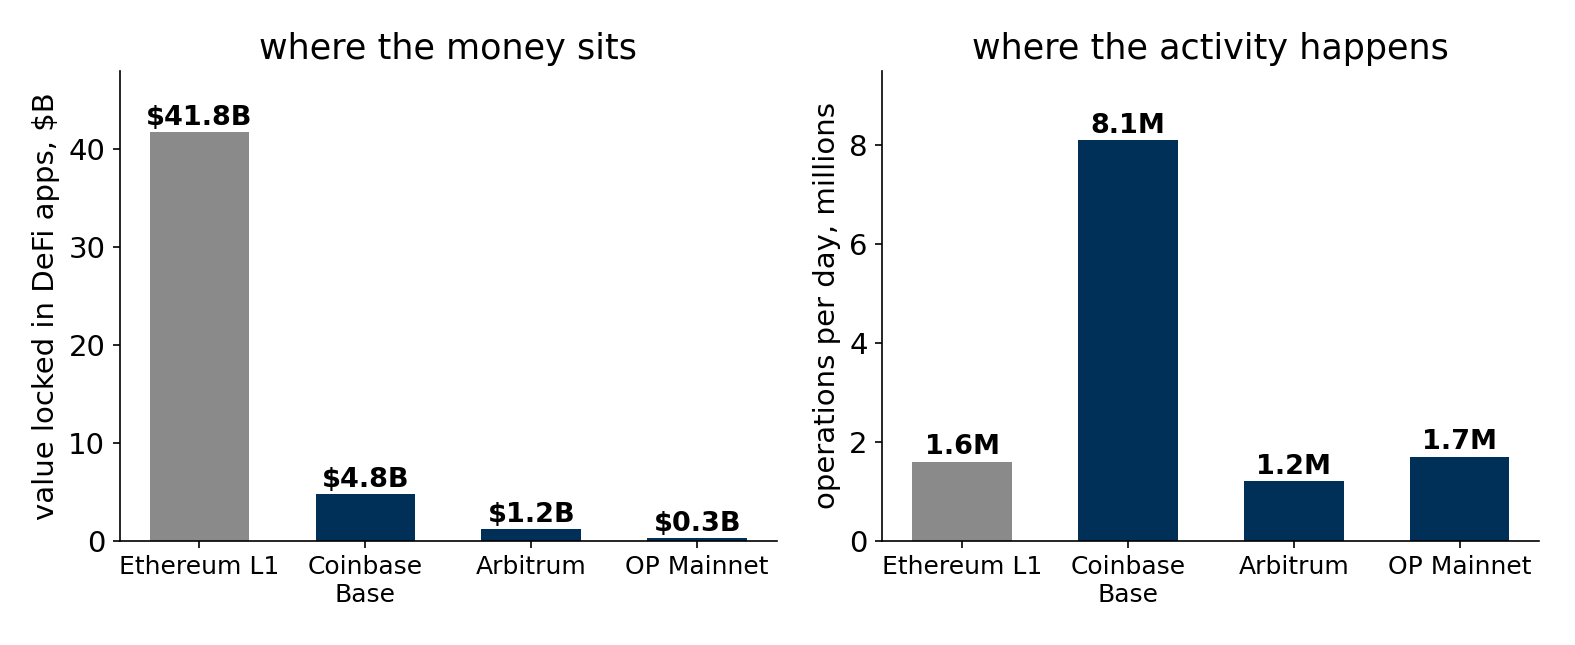
\includegraphics[width=0.88\textwidth]{fig_l2_share.png}
\end{center}
\vspace{-1mm}
{\small DefiLlama and L2BEAT APIs, Aug 2026; L1 activity approximate (Etherscan).}

\end{frame}


\section{Stablecoins}

\begin{frame}
\frametitle{What Is a Stablecoin?}
\small
\bi
\m A token defined by its peg -- a claim to a dollar, intended to always trade at a dollar 
\m So it is \textbf{not an asset class} -- appreciation is ruled out by construction. It is a \ul{transaction technology} for payments, savings, and smart-contract interoperability. (The cryptography is a mechanical design choice, \textbf{not} the source of value -- the peg is.) 
\m To an economist, a stablecoin is nothing new. \textbf{It is a bank deposit} -- but the issuer may or may not be a bank
\ei
\vspace{-1mm}
\begin{center}
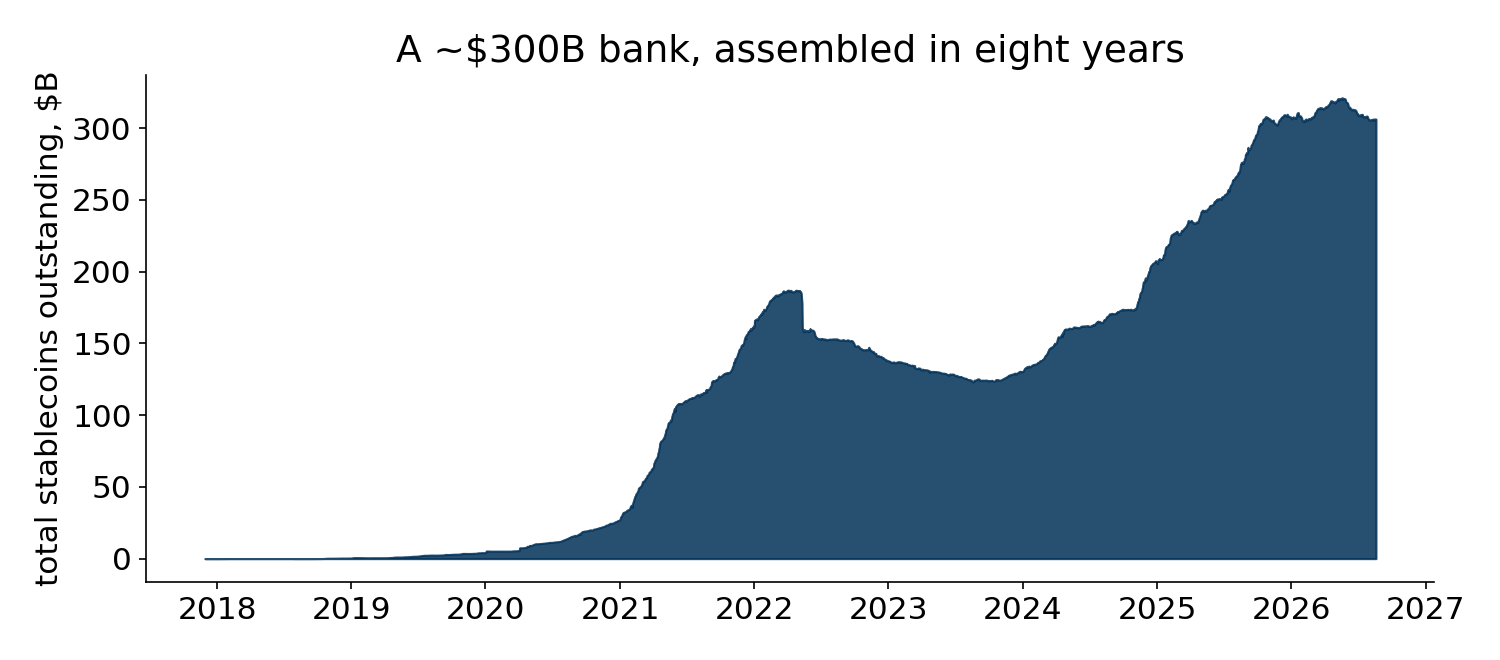
\includegraphics[width=0.52\textwidth]{fig_stablecoin_mcap.png}
\end{center}

\end{frame}

\begin{frame}
\frametitle{The Issuer Is a Bank in Everything but Name}
\begin{columns}
\column{0.42\textwidth}
\footnotesize
\bi
\m A pot of assets; tokens issued against it -- the holder is an \ul{uninsured depositor} 
\m Competition pushes for yield, meaning riskier collateral and thinner equity
\ei
\column{0.54\textwidth}
\begin{center}
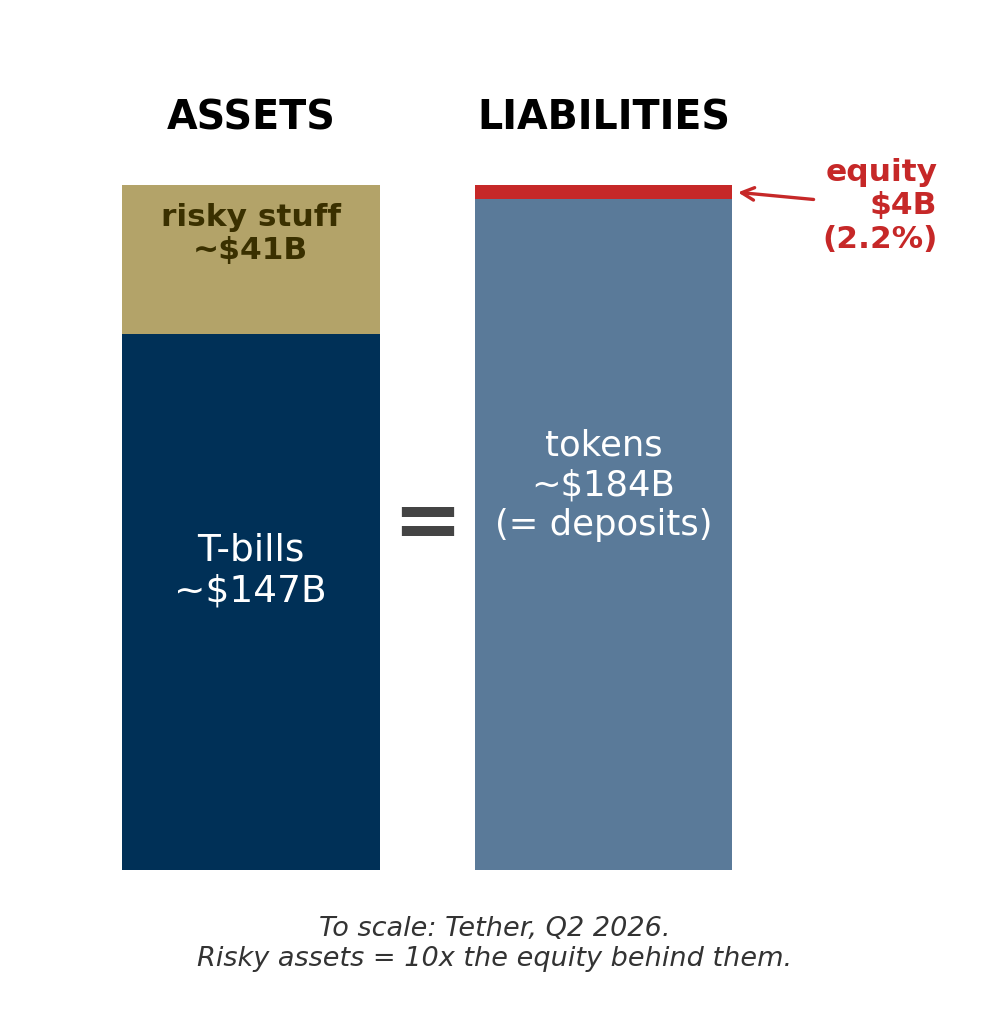
\includegraphics[height=0.82\textheight]{fig_issuer_balance_sheet.png}
\end{center}
\end{columns}
\end{frame}

\begin{frame}
\frametitle{And Bank-Like Liabilities Invite Bank-Like Runs}

\bi
\m A depositor who doubts the pot's value has one dominant move -- redeem first \pause
\m That is a \textbf{bank run} -- the same one that has stalked finance since the wildcat banking era \pause
\m We have already watched it happen. Terra/Luna (2022) collapsed in days; USDC broke its peg in the March 2023 SVB weekend before deposit insurance intervened 
\m The anatomy is documented. Terra's \$50B collapse in three days was a classic run led by large sophisticated holders (Liu, Makarov \& Schoar, NBER 2023); NY Fed work shows stablecoins behave like uninsured money-market funds under stress, with retail exiting after wholesale (Anadu et al.\ 2023; Luck's ``Historical Perspective on Stablecoins,'' 2025, draws the wildcat-era parallel directly)
\ei

\end{frame}

\begin{frame}
\frametitle{The GENIUS Act}

\bi
\m The 2025 GENIUS Act gives US stablecoins a banking-style rulebook of licensed issuers, reserve requirements, and disclosure \pause
\m One provision stands out. Issuers are \textbf{prohibited from paying interest} to holders \pause
\m So the product is \ul{a bank deposit that pays no interest} -- but with extra interoperability, because smart contracts can natively hold and accept it 
\m Demystified this way, the payments scorecard coming in Part II should not surprise you -- a zero-interest deposit competing against Treasuries, banks, and fast-payment rails has to win on convenience alone
\ei

\end{frame}

\begin{frame}
\frametitle{Stablecoins vs.\ Tokenized Deposits}

\bi
\m On the surface these are the same product -- a dollar claim that lives on a blockchain. The difference is \ul{where the money sits} \pause
\ei
\begin{center}
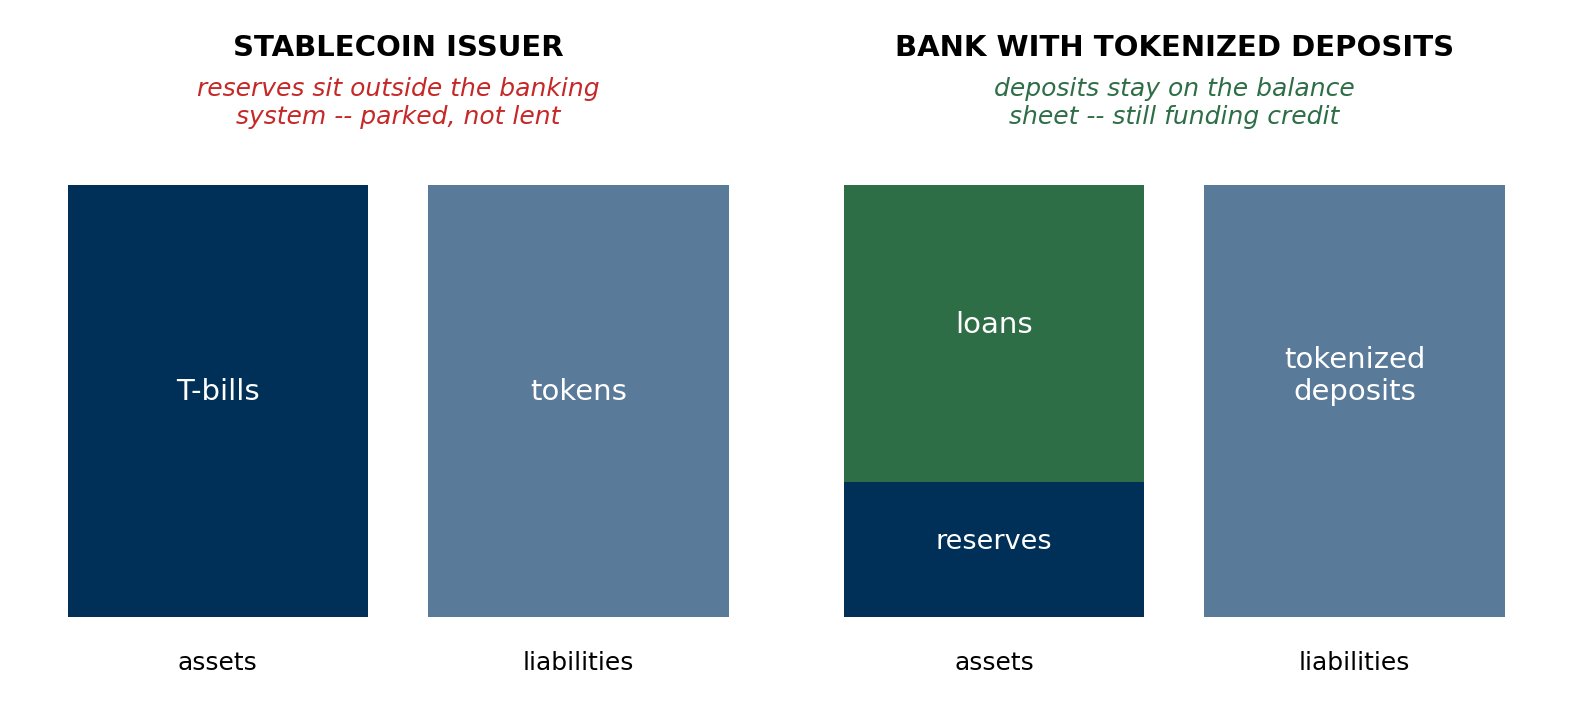
\includegraphics[width=0.72\textwidth]{fig_tokenized_deposits.png}
\end{center}
\vspace{-1mm}
{\small A dollar that migrates from a bank deposit into a stablecoin stops funding loans. At scale, that is \textbf{bank disintermediation} -- the policy fight underneath the stablecoin rulebook.}

\end{frame}

%----------------------------------------------------------------------------------------
%	PART II: THE STATE OF CRYPTO, AUGUST 2026
%----------------------------------------------------------------------------------------

\section{The State of Crypto, August 2026}

\begin{frame}
\frametitle{Part II. Where Does Crypto Actually Stand?}

\bi
\m Everything so far has been the \ul{technology} -- elegant, functional, mature \pause
\m Now the harder question. How is crypto doing as an \ul{industry}? \pause
\m My assessment: \\
\vspace{2mm}
\begin{center}
\textbf{Crypto has failed -- so far -- to mature into a product development platform for finance and software.}
\end{center}
\vspace{2mm} 
\m The next 30 minutes cover the evidence, five structural reasons, and what is thriving instead
\ei

\end{frame}

\begin{frame}
\frametitle{First, the Asset Everyone Asks About}
\begin{center}
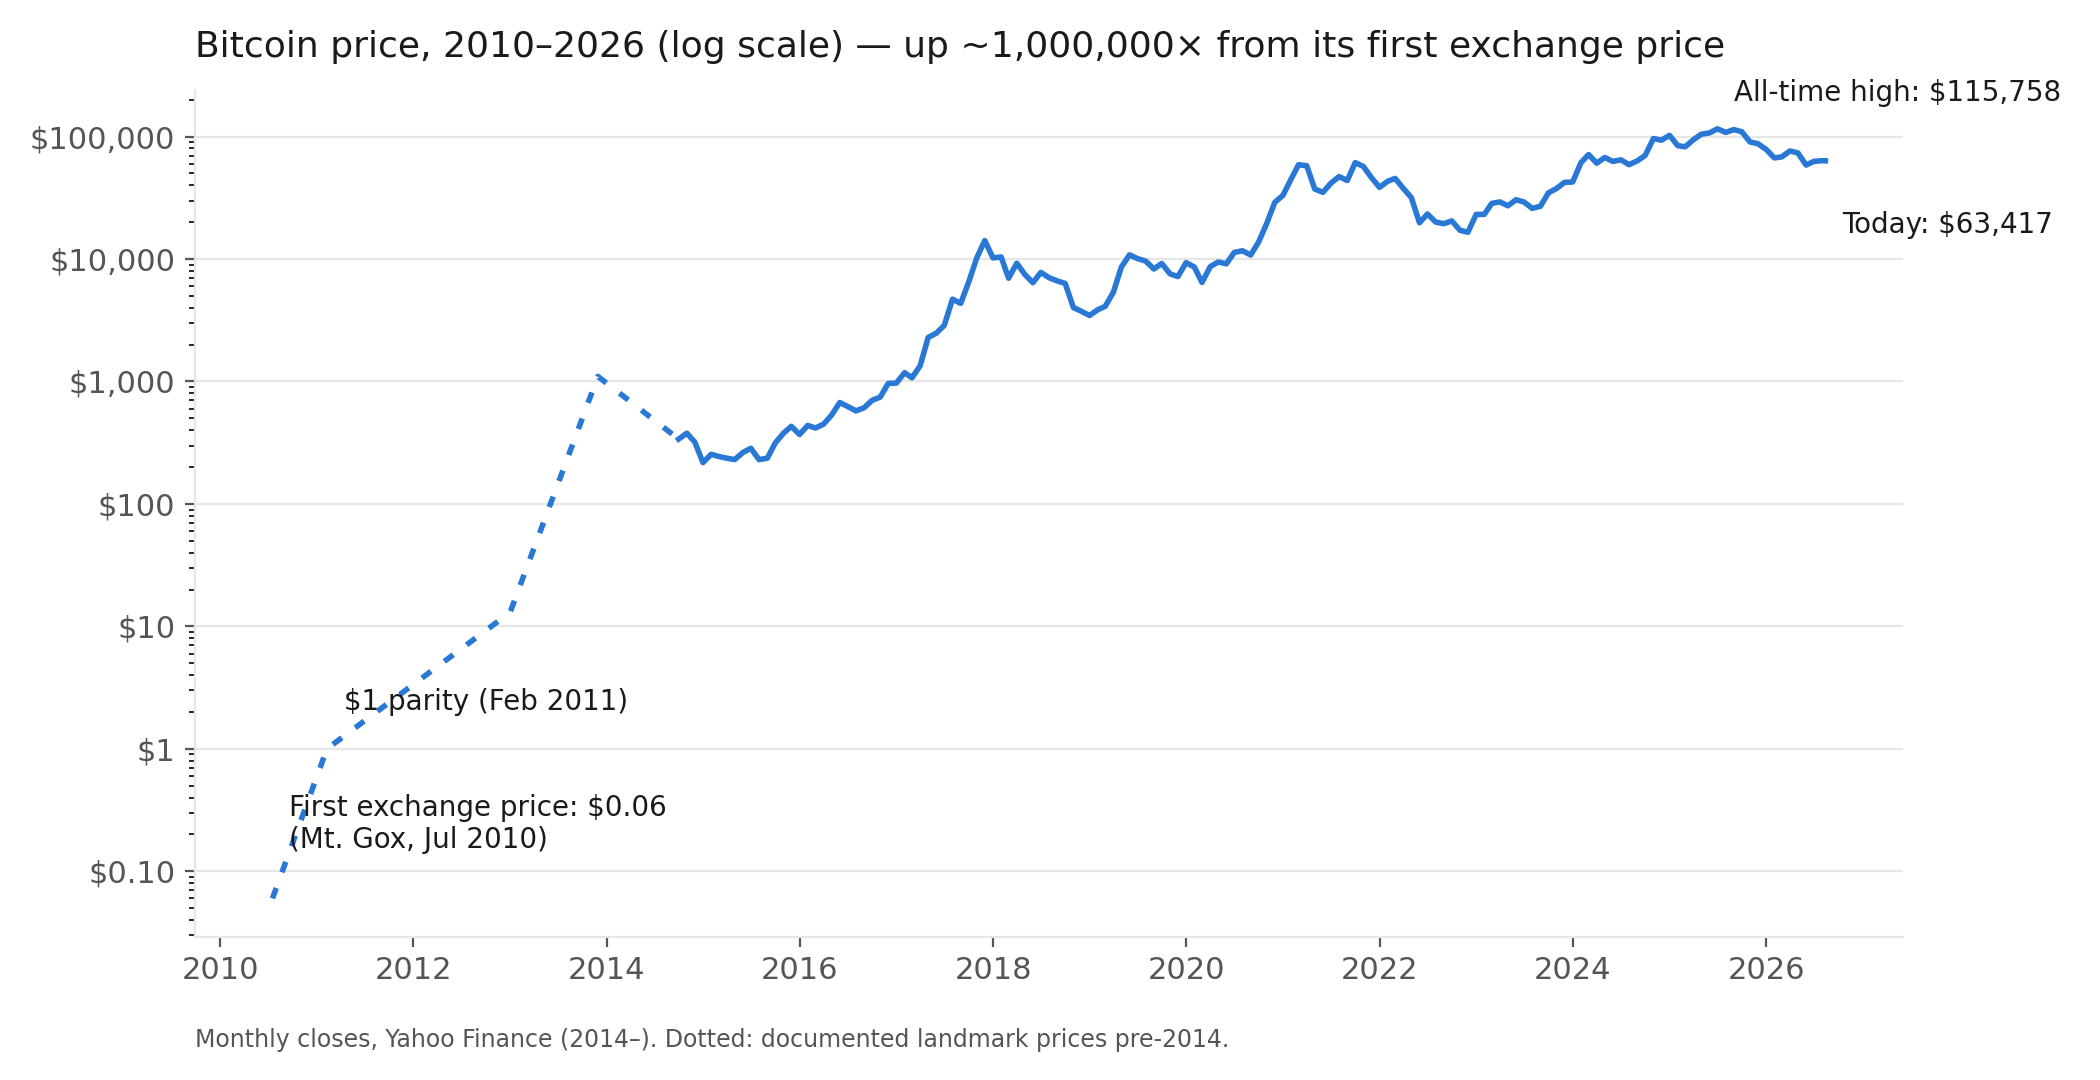
\includegraphics[width=0.84\textwidth]{fig_btc_log.png}
\end{center}
\vspace{-2mm}
{\small Both things are true at once. The greatest price appreciation of any asset in recorded history\ldots}
\end{frame}

\begin{frame}
\frametitle{\ldots and Traders' ``Price Halving'' Is a Regular Event}
\begin{center}
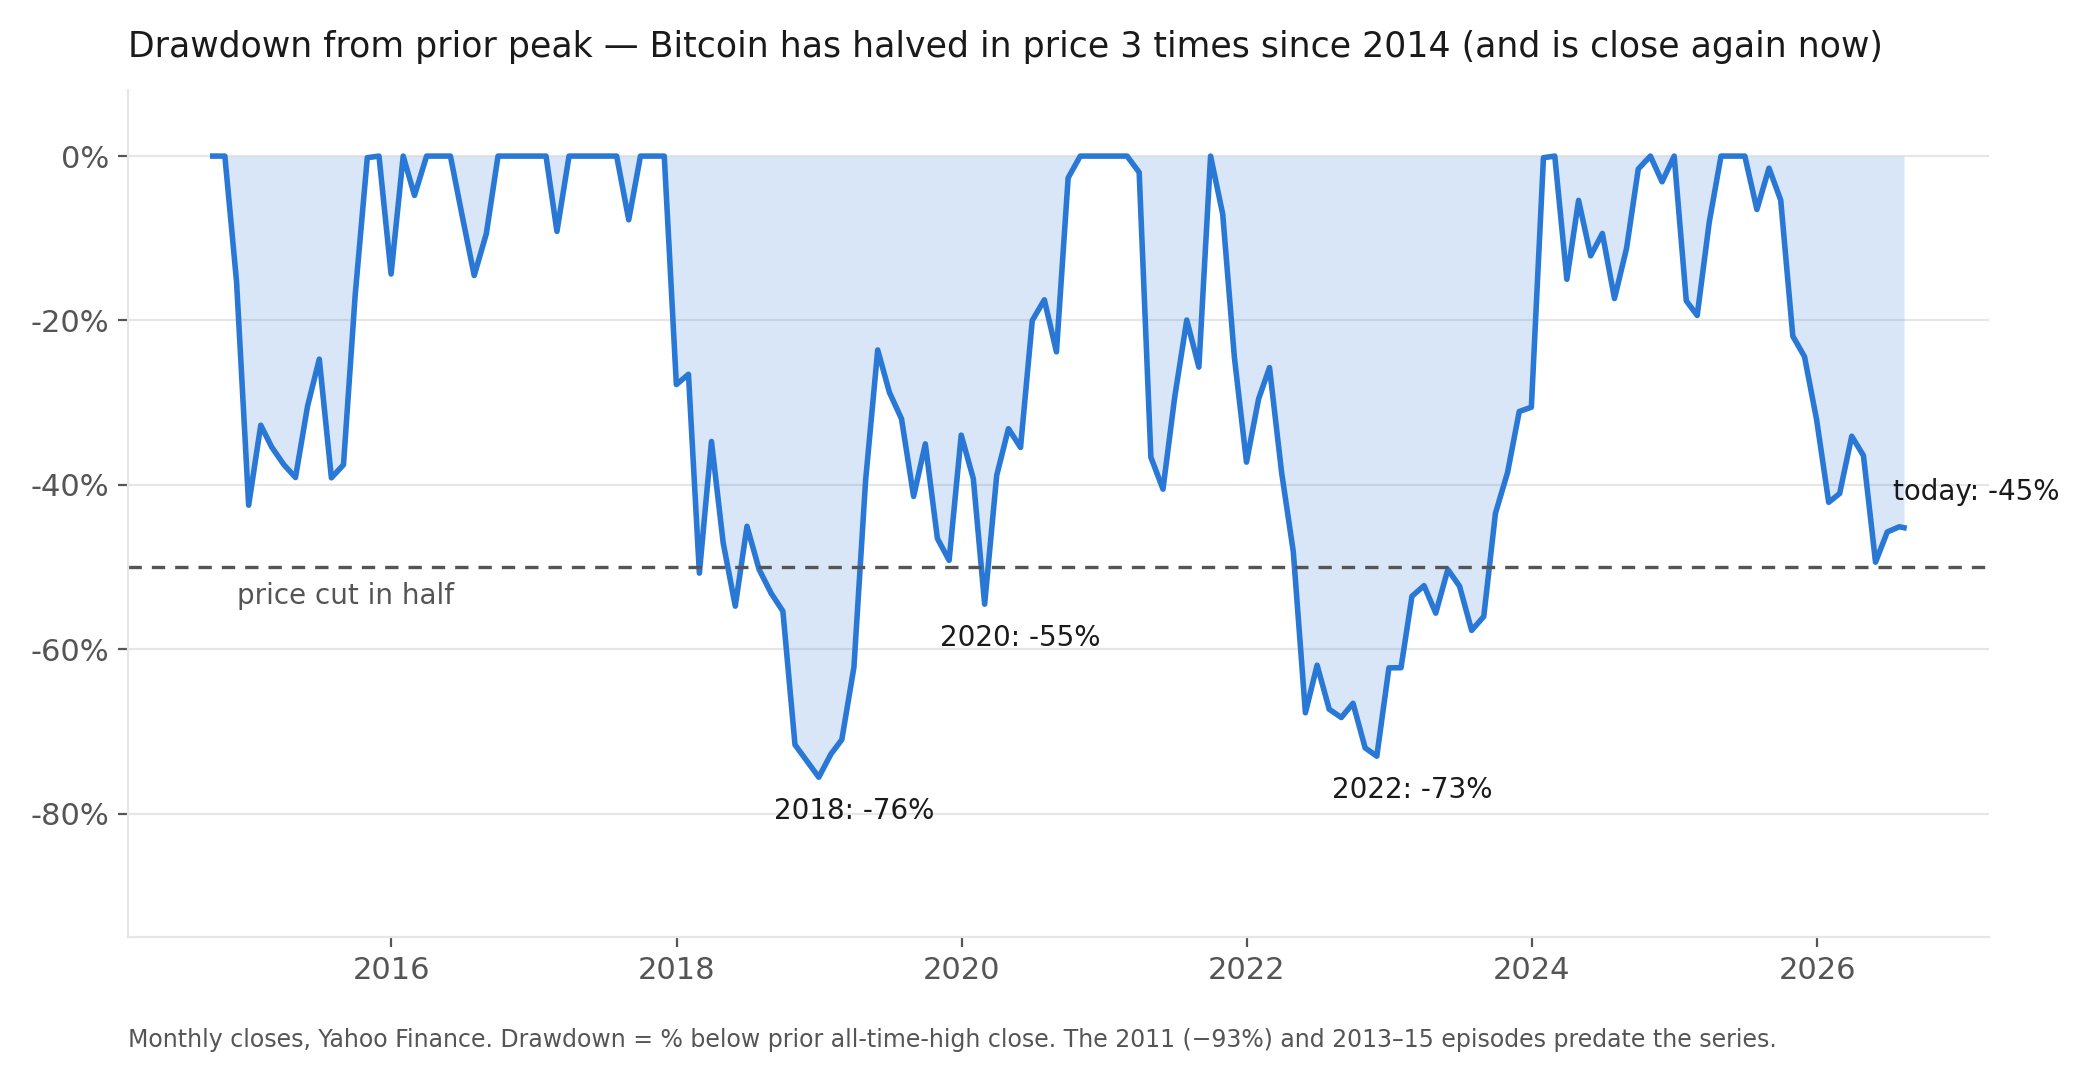
\includegraphics[width=0.84\textwidth]{fig_btc_drawdown.png}
\end{center}
\vspace{-2mm}
{\small Roughly every 2--4 years, Bitcoin loses half its value. Any portfolio thesis must survive this.}
\end{frame}

\begin{frame}
\frametitle{\ldots but Each Halving Happens at a Higher Floor}
\begin{center}
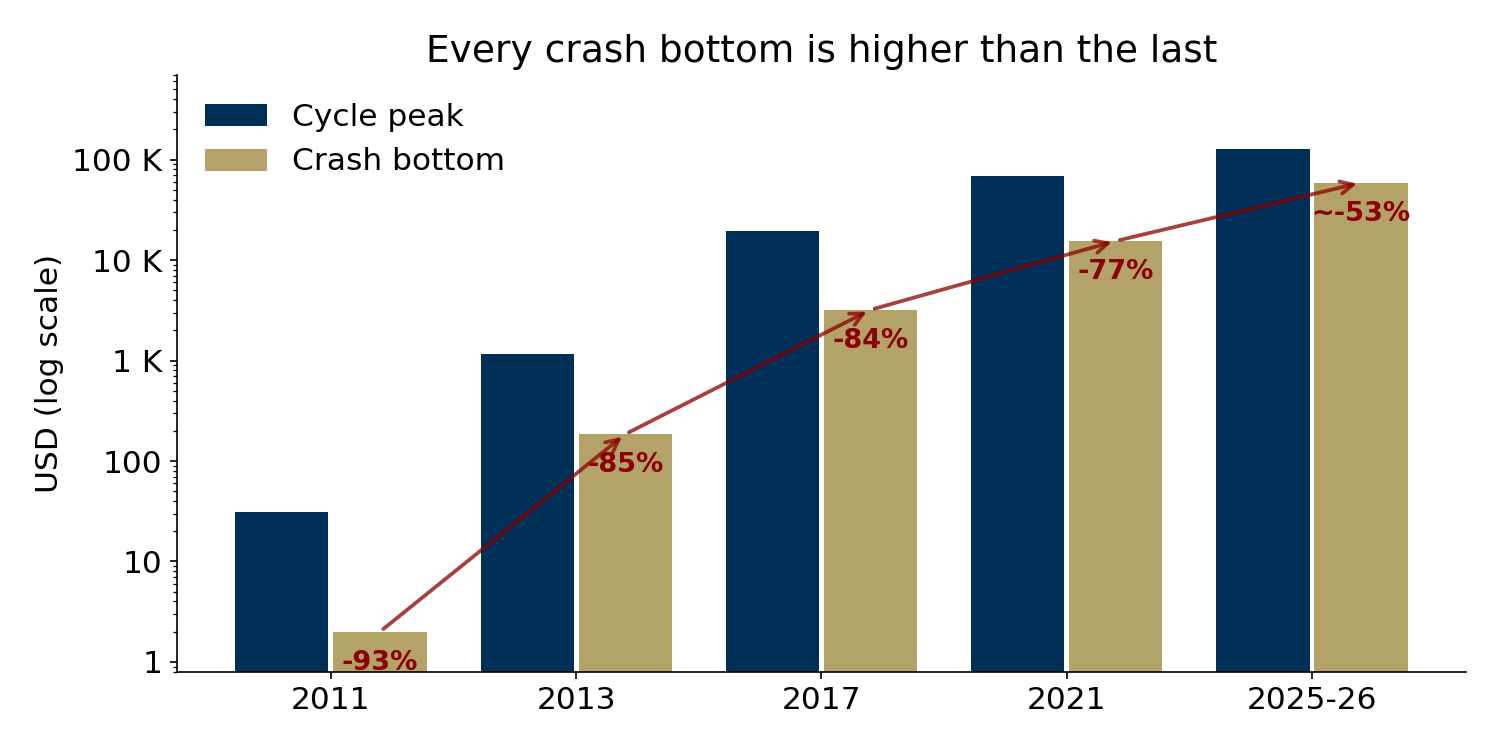
\includegraphics[width=0.72\textwidth]{fig_halving_floors.png}
\end{center}
\vspace{-2mm}
{\small The floor rises and the drawdowns shrink -- marked in red.}
\end{frame}

\begin{frame}
\frametitle{The Current Cycle}
\begin{center}
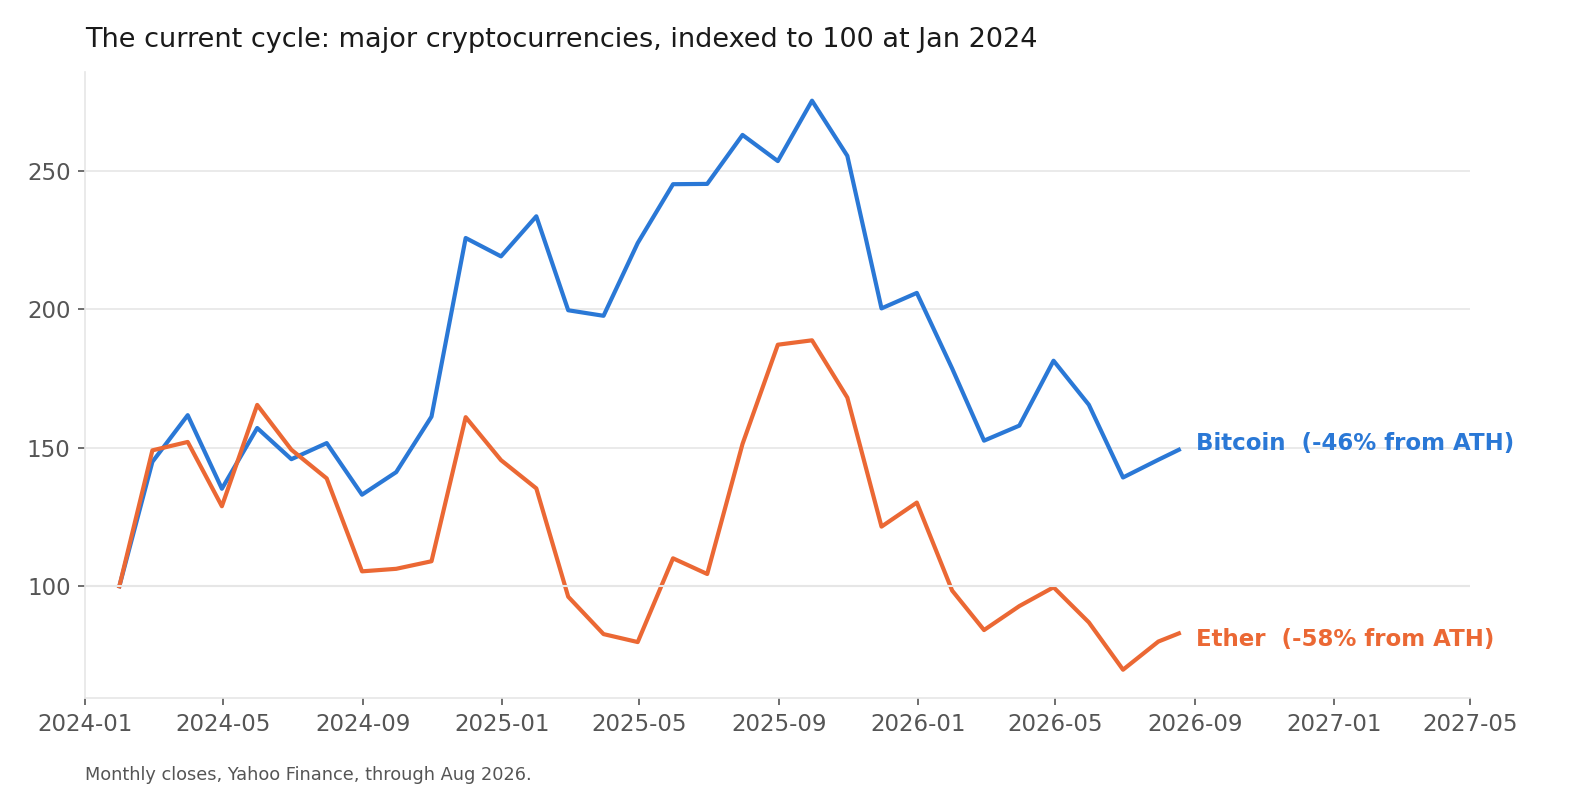
\includegraphics[width=0.85\textwidth]{fig_btc_recent.png}
\end{center}
\end{frame}

\begin{frame}
\frametitle{``Buy the Market''}

The CAPM says buy the market -- and BTC's market cap ($\sim$\$1.3T) is now roughly \alert{2.5\% of the S\&P 500's $\sim$\$55T} 

\begin{center}
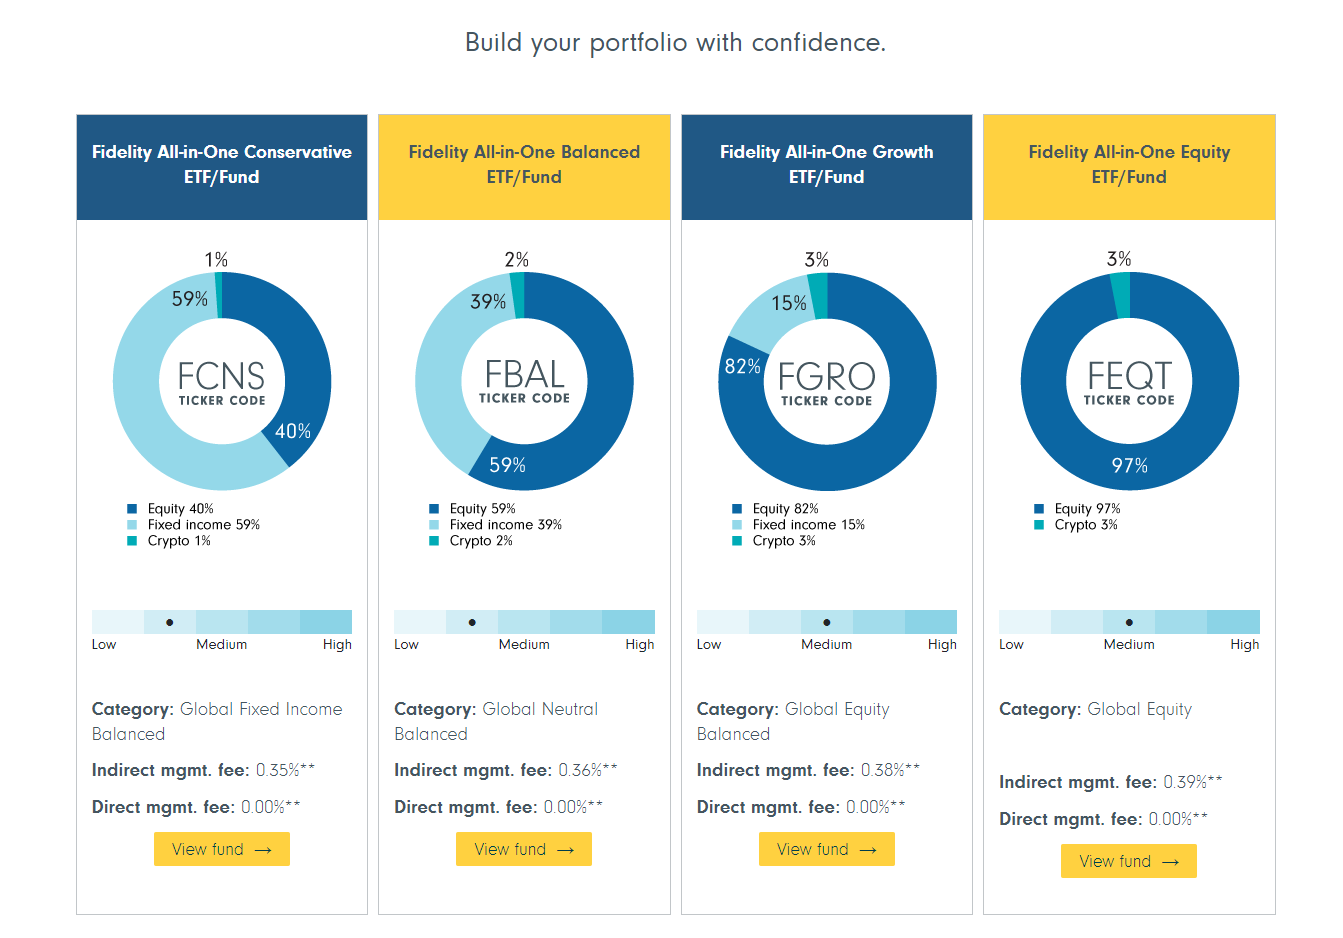
\includegraphics[width = 0.52\textwidth]{fig_fidelity.png}
\end{center} 

\vspace{1ex}
\scriptsize
\href{https://www.fidelity.ca/en/investments/solutions-portfolios/all-in-one/}{Fidelity Canada}; market caps as of August 2026 (CoinGecko; S\&P DJI).

\end{frame}

\begin{frame}{The ``Market Cap'' Illusion}

\textbf{Market Capitalization} is just units outstanding times unit price 

\bi 
\m Say everyone tried to sell their BTC tomorrow. Would they get that price for it? \pause 
\m Traditional assets (stocks, bonds) generate \textbf{dividends} or \textbf{coupons} 
\bi 
\m If a major owner of a stock worth 2\% of the S\&P500 sold, the supply would be absorbed relatively quickly 
\m Investors are willing to substitute frictionlessly between stocks if one is temporarily undervalued \pause 
\ei 
\m Reports of \$TRUMP being worth \$10 billion+ assume unit price would survive a large selloff (a bad assumption in my opinion) 
\ei 
    
\end{frame}

\begin{frame}
\frametitle{The Long-Run Quantum Risk}
\bi
\m Bitcoin's signatures rest on the discrete-log problem (recall ElGamal) -- and quantum computers solve discrete logs efficiently in theory (Shor's algorithm) 
\ei
\begin{center}
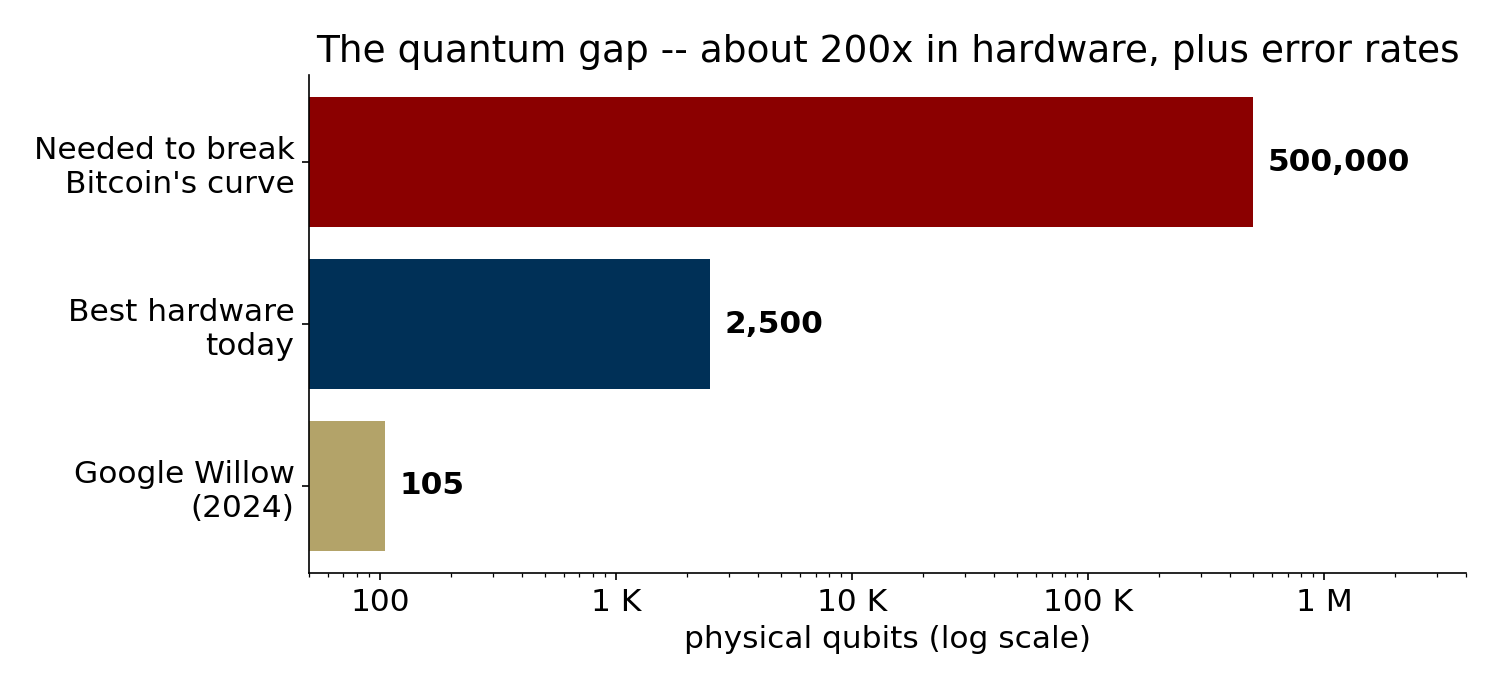
\includegraphics[width=0.66\textwidth]{fig_quantum_gap.png}
\end{center}
\vspace{-2mm}
{\small Expert projections (not facts) put cryptographically relevant machines in the \textbf{2030s}. Quantum-resistant cryptography already exists -- but migrating the chain to it is a massive coordination problem.}
\end{frame}

\begin{frame}
\frametitle{The Payments Scorecard}

After 17 years, here is crypto's share of the job it was invented for.
\small
\bi
\m The stablecoin share, drawn to scale (and essentially \textbf{0\%} of wholesale) \ldots
\begin{center}
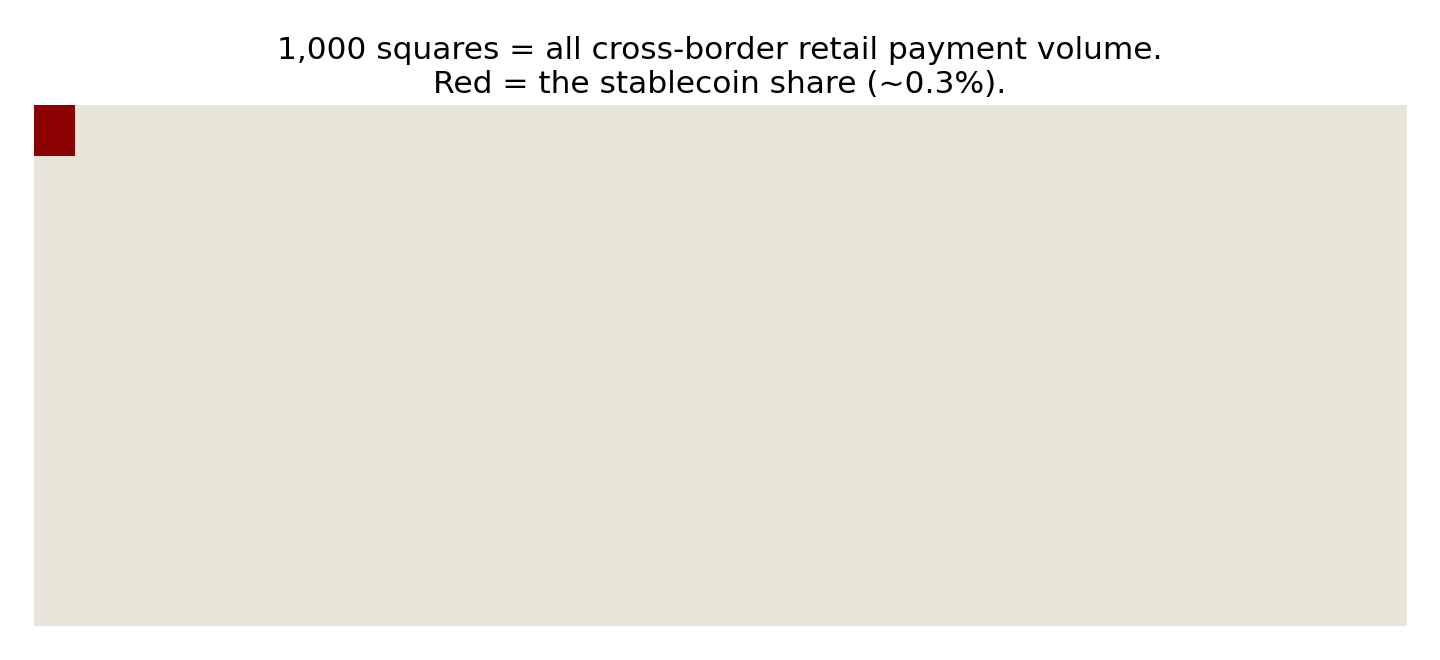
\includegraphics[width=0.50\textwidth]{fig_stablecoin_share.png}
\end{center} \pause
\m Banca d'Italia ran actual \$200 remittances (USDC vs.\ traditional corridors) and found \textbf{no systematic cost or speed advantage} once on/off-ramps are counted. Growth continues -- from a base that rounds to zero
\ei
\vfill
{\tiny FXC Intelligence--Allium (July 2026); Banca d'Italia stablecoin-remittance study (August 2026).}

\end{frame}

\begin{frame}
\frametitle{The Flagship Issuer}
\begin{columns}
\column{0.62\textwidth}
\footnotesize
\bi
\m Tether (USDT), the largest issuer, saw equity fall \textbf{a third} in two quarters 
\m The cushion sits under the risky slice of the Part I balance sheet 
\m Where usage is growing fastest -- emerging markets -- the IMF warns of \ul{dollarization} (residents abandoning the local currency for dollar claims) and illegal-payment channels (Nigeria note, July 2026) 
\m The largest exchange, Binance, pled guilty (2023) to Bank Secrecy Act and sanctions violations, paying \textbf{\$4.3B} and exiting the US market
\bi
\m Since the settlement, $>$\$1B in Iran-linked flows, under active DOJ monitorship
\ei
\ei
\column{0.34\textwidth}
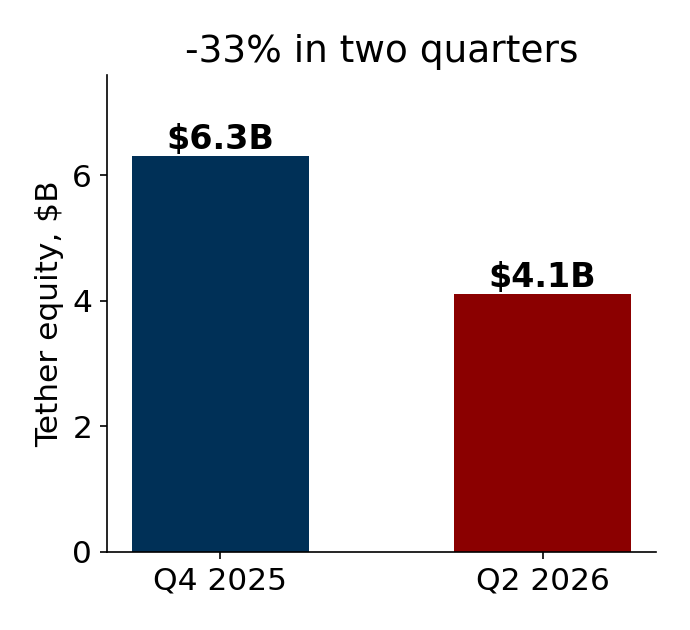
\includegraphics[width=\textwidth]{fig_tether_equity.png}
\end{columns}
\vfill
{\scriptsize Tether attestation, Q2 2026; IMF Note on Nigeria's cross-border crypto flows (July 2026); Fortune, Senate HSGAC letter (Feb--Apr 2026).}

\end{frame}

\begin{frame}
\frametitle{In Their Own Words}

From the unsealed CFTC and SEC complaints against Binance (2023): \pause
\vspace{2mm}
\bi
\m Binance's Chief Compliance Officer, on certain customers: \\ \emph{``Like come on. They are here for crime.''} \pause
\m Binance's Money Laundering Reporting Officer, in reply: \\ \emph{``we see the bad, but we close 2 eyes''} 
\m The CCO again, December 2018: \\ \emph{``we are operating as a fking unlicensed securities exchange in the USA bro''}
\ei
\vfill
{\scriptsize CFTC v.\ Zhao, Binance \& Lim, complaint filed Mar 27, 2023 (N.D. Ill.); SEC v.\ Binance, complaint filed June 5, 2023. Quotes verbatim from the complaints.}

\end{frame}

\begin{frame}
\frametitle{The Platform Thesis (As Designed)}

How crypto was \ul{supposed} to become a product platform \ldots
\bi
\m The \textbf{utility-token thesis} says a token's value grows in proportion to the use cases built on its platform
\bi
\m Monegro's \href{https://www.usv.com/writing/2016/08/fat-protocols/}{``Fat Protocols''} (2016) argued that, unlike the internet (where value went to apps, not TCP/IP), blockchain value would concentrate in the \ul{protocol layer} -- so hold the token \pause
\m Burniske's MV=PQ valuation says a token's price should scale with the transaction volume its platform hosts \pause
\m Cong, Li \& Wang's \emph{Tokenomics} (RFS 2021) formalized it, deriving token prices from platform adoption
\ei 
\m This thesis is exactly why DAO treasuries look the way they do \ldots
\bi
\m Hold billions in native tokens $\rightarrow$ write grants to developers $\rightarrow$ developers build DApps $\rightarrow$ usage raises token value $\rightarrow$ treasury appreciates
\ei 
\m A flywheel, on paper.  \textbf{The flywheel never spun.} Five reasons why $\rightarrow$
\ei

\end{frame}

\begin{frame}
\frametitle{Reason 1. Open Design Invites Predators}
\small
\bi
\m Permissionless + irreversible + pseudonymous means no chargebacks, no deposit insurance, no intermediary with a duty to you
\m The retail-scale version is the \textbf{rug pull} -- launch a token, attract buyers, drain the liquidity, vanish
\ei
\begin{columns}
\column{0.58\textwidth}
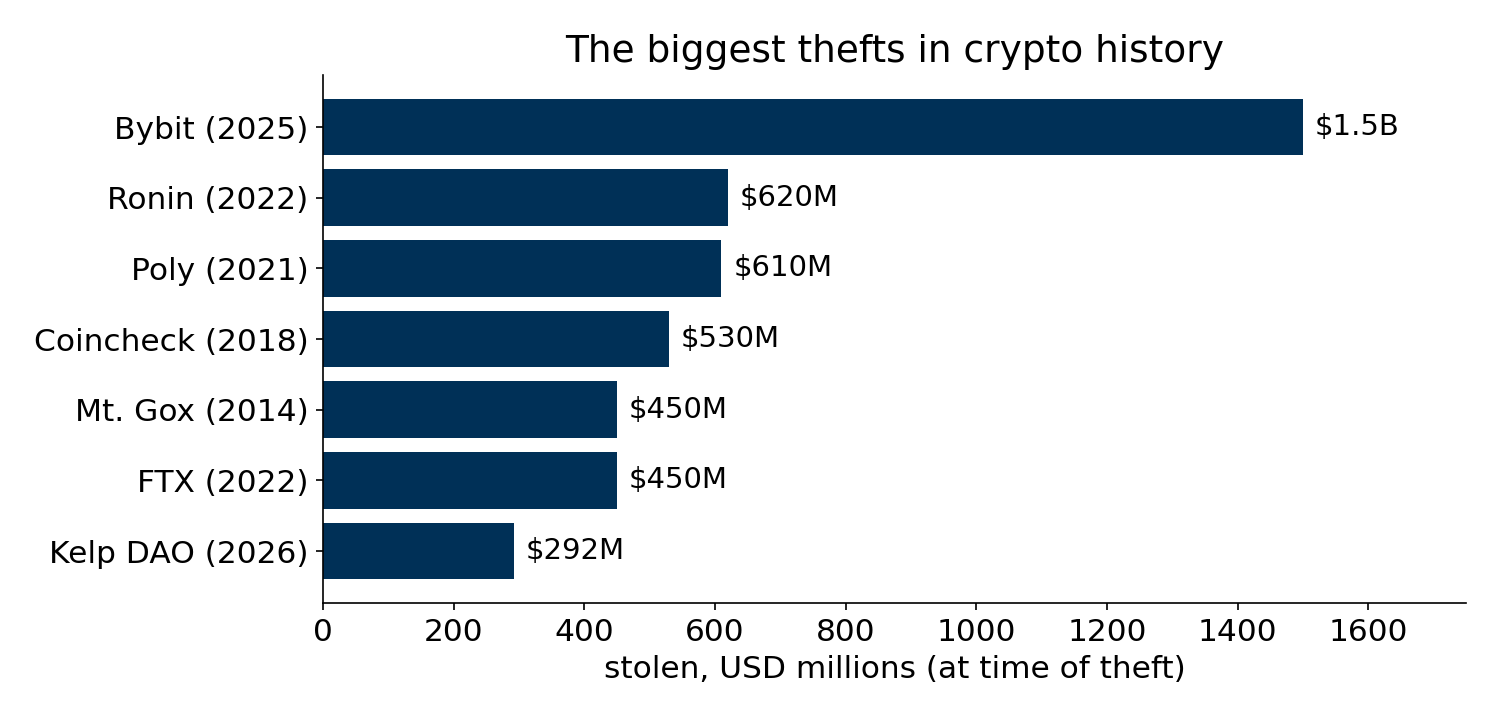
\includegraphics[width=0.95\textwidth]{fig_hacks.png}
\column{0.36\textwidth}
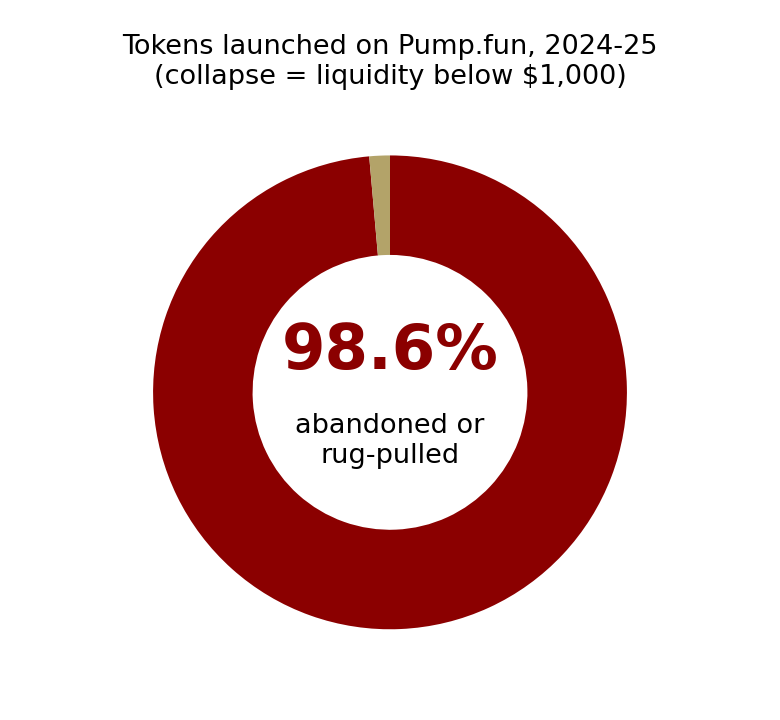
\includegraphics[width=0.92\textwidth]{fig_rugpull_donut.png}
\end{columns}
\vspace{1mm}
{\small Even on Arbitrum -- the most trusted L2 -- protocols were drained in 2026 (Kelp DAO, above). The openness that makes the technology beautiful makes the \ul{industry} adversarial.}
\end{frame}

\begin{frame}
\frametitle{Reason 2. A Tragedy of the Commons}

\bi
\m The developer who builds a great DApp creates value for every token holder -- but captures almost none of it \pause
\m Under equity, building a great product inside a firm means the shareholders (including you, via options) capture it \pause
\m Token grants $\neq$ equity; they are one-time payments with no claim on the value your app creates going forward 
\m The prediction is \textbf{persistent underinvestment} in the ecosystem -- exactly what we observe 
\m {\small (This is the subject of an ongoing Harvard Business School case study I'm coauthoring.)}
\ei

\end{frame}

\begin{frame}
\frametitle{Reason 3. Nobody Touches the Chain}

\bi
\m Most people will never manage keys, gas, or slippage -- they interface through a polished app that abstracts many layers over the blockchain \pause
\m So the \ul{app layer} owns the customer relationship, the data, and the margin \pause
\m In practice Monegro's ``fat protocols'' thesis inverted. The value accrued to Coinbase -- the app layer -- not to the protocols 
\m A platform whose end users can't touch it directly is a platform whose token can't capture their value
\ei

\end{frame}

\begin{frame}
\frametitle{Reason 4. The Talent Sorted}

\bi
\m \textbf{My own assessment}: \pause
\m The best and most trustworthy developers have been content to pay the regulation-and-taxation toll to build inside Uncle Sam's dollar-denominated, SEC-regulated ecosystem \pause
\m Bad actors find the unregulated setup optimal for scamming -- so they stayed 
\m A sorting equilibrium set in. Over time, ``crypto-native'' became a negative quality signal for talent and users alike 
\m Once sorting sets in, it self-reinforces, as users learn to distrust, honest builders leave faster
\ei

\end{frame}

\begin{frame}
\frametitle{Reason 5. Anonymity Meets AI}

\bi
\m From my research with Victor Huang on the Arbitrum DAO, whose treasury holds billions of dollars \pause
\m Forum deliberation predicted vote outcomes -- until early 2024, when LLMs could produce indistinguishable governance prose \pause
\m After that, the correlation is \textbf{gone} -- even though few posts were actually AI-written 
\m The theory is that when identity is anonymous and text is cheap to fake, the signal value of all text can collapse at a discrete tipping point 
\m Anonymity -- a design pillar of crypto -- is precisely the vulnerability AI exploits
\ei
\vfill
{\scriptsize Hall \& Huang, ``The Effect of AI Writing on Governance: Evidence from a \$3.5 Billion DAO'' (working paper) -- josephphall.com.}

\end{frame}

\begin{frame}
\frametitle{AI's Second Squeeze Is in Hardware}
\begin{center}
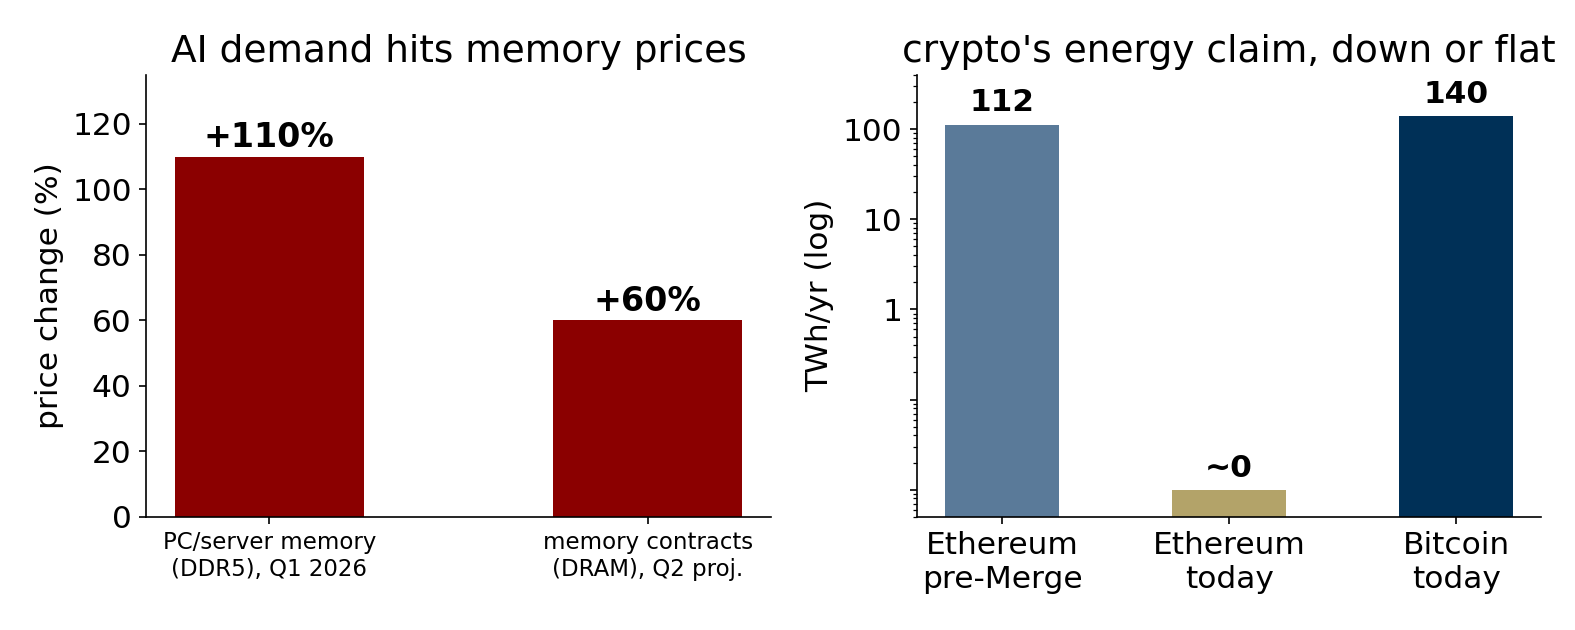
\includegraphics[width=0.72\textwidth]{fig_hardware_squeeze.png}
\end{center}
\vspace{-2mm}
\small
\bi
\m Miners are converting. IREN, a large listed bitcoin miner, raised \$3B to turn mining sites into AI data centers \pause
\m The energy decline is by design -- mining burn is socially wasteful; ending it was the point of The Merge and of L2s. Mining secured the chain because it was the best use of that hardware. It no longer is.
\ei
\vfill
{\tiny TrendForce DRAM contract data Q1--Q2 2026; ethereum.org (Merge); Cambridge CBECI; IREN convertible notes (May 2026).}
\end{frame}

\begin{frame}
\frametitle{Meanwhile, TradFi Is Adopting the Technology}

The blockchain applications are thriving -- inside the regulated system.
\bi
\m \textbf{Robinhood moved its backend onto a blockchain}. Robinhood Chain (mainnet July 2026), built on Arbitrum's stack -- tokenized U.S.\ stocks trading 24/7 in 120+ countries \pause
\bi
\m Caveat: the ``stock tokens'' are debt claims on Robinhood, not equity \pause
\ei
\m \textbf{Native tokenized securities}. JPMorgan, BlackRock \& Goldman tokenizing stocks and Treasuries -- the actual asset, not a wrapper; BNY pushing 24/7 Treasury settlement 
\m \textbf{Tokenized deposits}. Wells Fargo and other major banks, for corporate treasury 
\m Note what they kept (the ledger, atomic settlement, programmability) and what they dropped (permissionlessness, anonymity, the native token)
\ei
\vfill
{\scriptsize Robinhood newsroom (Jun 2025); Forbes, CoinDesk (Feb--Jul 2026); WSJ (Jul--Aug 2026).}

\end{frame}

\begin{frame}
\frametitle{\ldots and Sovereigns Are Building the Rails}

\bi
\small
\m \textbf{Tokenized sovereign debt}. UK digital gilt pilot (HSBC/LSEG), first digital bond by 2027 \pause
\m \textbf{Central-bank digital currency (CBDC) pilots}. ECB digital-euro pilot (36 payment firms); Korea's two-layer CBDC; BIS Project Agor\'a for programmable cross-border payments \pause
\m \textbf{Public fast payments winning at scale}. Brazil's Pix so dominant it triggered a US trade dispute; BRICS cross-border linkage; e-CNY settling cross-border trades in 30 minutes 
\m Across all of these, the state and the banks took what worked and put it behind identity, regulation, and the sovereign's monetary fiat
\ei

\end{frame}

\begin{frame}
\frametitle{Testing ``Bitcoin Is a Bet Against Fiat''}

\bi
\m If BTC hedges sovereign money-printing, it should rise on \ul{inflation surprises}. Monthly data, 2014--2026.
\ei
\begin{center}
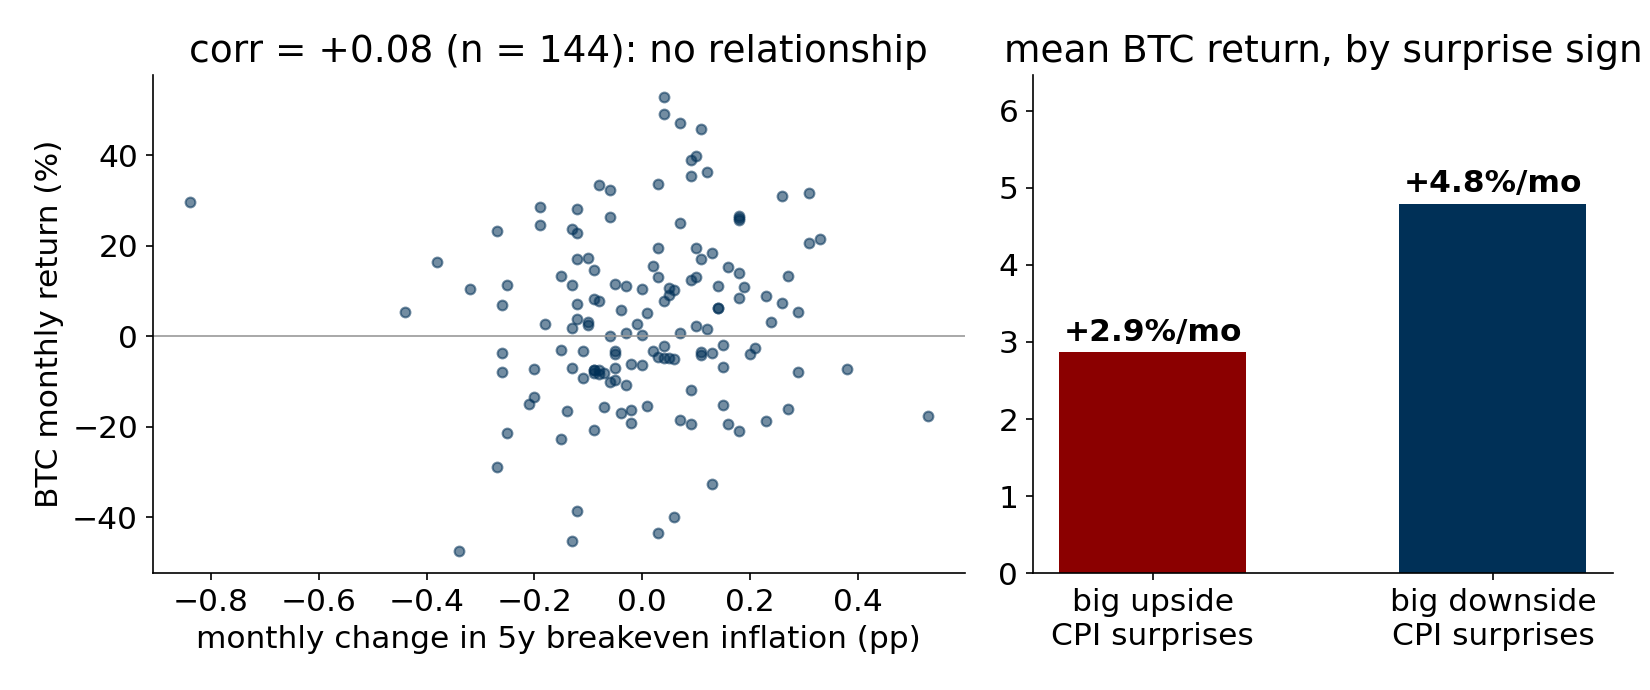
\includegraphics[width=0.74\textwidth]{fig_inflation_hedge.png}
\end{center}
\vspace{-2mm}
{\footnotesize And in the one real test -- the 2021--22 CPI shock, the largest inflation surprise in four decades -- BTC returned \alert{$-$59\%}. Where fiat \ul{does} fail (Nigeria, Argentina), the flight is into \ul{dollar stablecoins}. The debasement hedge exists, and it is the dollar.}

\end{frame}

\begin{frame}{Faster Horses}
\centering
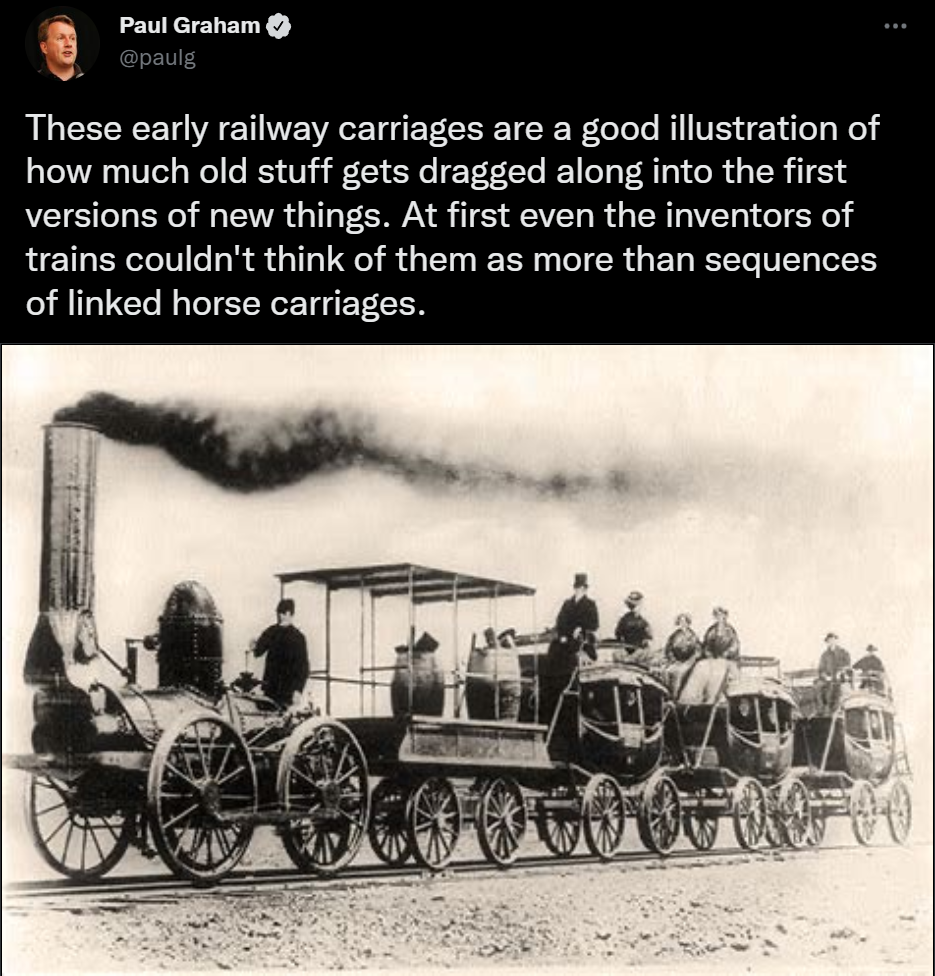
\includegraphics[height=0.85\textheight]{fig_faster_horses.png}

\end{frame}

\begin{frame}
\frametitle{Prognosis. Augmentation, Not Replacement}

\bi
\m The libertarian wild-west utopia -- money and finance without states, banks, or identity -- has not come to pass, and looks less like a forecast and more like science fiction every year \pause
\m \textbf{That is not a doomer take on the technology.} The blockchain toolkit -- shared ledgers, atomic settlement, programmable assets, 24/7 markets -- is proving genuinely transformative in TradFi's hands \pause
\m Crypto will not \ul{replace} the traditional financial system; on current evidence it will \ul{augment and support} it -- the rails beneath tokenized Treasuries, stock tokens, and instant settlement 
\m The five structural problems explain why the value migrated. They are design features of permissionless anonymity, and TradFi adopted everything else 
\m As a steelman, crypto has been declared dead before, and EM stablecoin demand is real. What would change my mind? A DApp ecosystem that grows without grant subsidies.
\ei

\end{frame}

\begin{frame}
\frametitle{Discussion}

\begin{center}
{\Large Questions to argue about}
\end{center}
\vspace{3mm}
\bi
\m If the utility-token flywheel can't spin, what should a DAO do with a multi-billion-dollar treasury? Is there a mechanism design that lets DApp developers capture the value they create? \pause
\m Is there a market for proof of computing power in the long run? Is Bitcoin that market? \pause
\m How long will the U.S. dollar stay the world's dominant currency? Will it be replaced by another sovereign or by something else?
\ei

\end{frame}

\begin{frame}
\frametitle{Credits \& Sources}

\begin{columns}
\column{0.72\textwidth}
\bi
\m Part I is adapted in part from teaching materials by \textbf{Anthony Lee Zhang}, used with permission -- thank you, Anthony
\m Much of the market evidence in Part II was surfaced through \textbf{Darrell Duffie}'s fast-digital-payments seminar list
\m Research cited includes Hall \& Huang (2026); Cong, Li \& Wang (RFS 2021); Monegro (2016); reports by FXC Intelligence--Allium, Banca d'Italia, the BIS, and the IMF (2026)
\m Price data from Yahoo Finance. Errors and opinions are mine alone.
\ei
\column{0.24\textwidth}
\begin{center}

\includegraphics[width=\textwidth]{fig_qr_site.png}\\[0.5mm]
{\small josephphall.com}
\end{center}
\end{columns}

\end{frame}






%------------------------------------------------


\end{document}